\documentclass[12pt,cmcyralt]{article}
\usepackage{cmap}
\usepackage[T2A]{fontenc}
\usepackage[utf8]{inputenc}
\usepackage[russian]{babel}
\usepackage{graphicx}
\usepackage{amsthm,amsmath,amssymb}
\usepackage[russian,colorlinks=true,urlcolor=red,linkcolor=blue]{hyperref}
\usepackage{enumerate}
\usepackage{datetime}
\usepackage{fancyhdr}
\usepackage{lastpage}
\usepackage{color}
\usepackage{verbatim}
\usepackage{tikz}
\usepackage{epstopdf}
\usepackage{xifthen}
\usepackage{float}
\usepackage{xcolor}
\usepackage{hyperref}

\definecolor{linkcolor}{HTML}{799B03} % цвет ссылок
\definecolor{urlcolor}{HTML}{799B03} % цвет гиперссылок
 
\hypersetup{pdfstartview=FitH,  linkcolor=linkcolor,urlcolor=urlcolor, colorlinks=true}

\parskip=0em
\parindent=0em

\sloppy
\voffset=-20mm
\textheight=235mm
\hoffset=-25mm
\textwidth=180mm
\headsep=12pt
\footskip=20pt

\setcounter{page}{0}
\pagestyle{empty}

% Основные математические символы
\DeclareSymbolFont{extraup}{U}{zavm}{m}{n}
\DeclareMathSymbol{\heart}{\mathalpha}{extraup}{86}
\newcommand{\N}{\mathbb{N}}   % Natural numbers
\newcommand{\R}{\mathbb{R}}   % Ratio numbers
\newcommand{\Z}{\mathbb{Z}}   % Integer numbers
\def\EPS{\varepsilon}         %
\def\SO{\Rightarrow}          % =>
\def\EQ{\Leftrightarrow}      % <=>
\def\t{\texttt}               % mono font
\def\c#1{{\rm\sc{#1}}}        % font for classes NP, SAT, etc
\def\O{\mathcal{O}}           %
\def\NO{\t{\#}}               % #
\renewcommand{\le}{\leqslant} % <=, beauty
\renewcommand{\ge}{\geqslant} % >=, beauty
\def\XOR{\text{ {\raisebox{-2pt}{\ensuremath{\Hat{}}}} }}
\newcommand{\q}[1]{\langle #1 \rangle}               % <x>
\newcommand\URL[1]{{\footnotesize{\url{#1}}}}        %
\newcommand{\sfrac}[2]{{\scriptstyle\frac{#1}{#2}}}  % Очень маленькая дробь
\newcommand{\mfrac}[2]{{\textstyle\frac{#1}{#2}}}    % Небольшая дробь
\newcommand{\score}[1]{{\bf\color{red}{(#1)}}}

% Отступы
\def\makeparindent{\hspace*{\parindent}}
\def\up{\vspace*{-0.3em}}
\def\down{\vspace*{0.3em}}
\def\LINE{\vspace*{-1em}\noindent \underline{\hbox to 1\textwidth{{ } \hfil{ } \hfil{ } }}}
%\def\up{\vspace*{-\baselineskip}}

\lhead{Дискретная математика}
\chead{}
\rhead{Лекции \CURNO. \NAME.}
\renewcommand{\headrulewidth}{0.4pt}

\lfoot{}
\cfoot{\thepage\t{/}\pageref*{LastPage}}
\rfoot{}
\renewcommand{\footrulewidth}{0.4pt}

\newenvironment{MyList}[1][4pt]{
  \begin{enumerate}[1.]
  \setlength{\parskip}{0pt}
  \setlength{\itemsep}{#1}
}{       
  \end{enumerate}
}
\newenvironment{InnerMyList}[1][0pt]{
  \vspace*{-0.5em}
  \begin{enumerate}[a)]
  \setlength{\parskip}{#1}
  \setlength{\itemsep}{0pt}
}{
  \end{enumerate}
}

\newcommand{\Section}[1]{
  \refstepcounter{section}
  \addcontentsline{toc}{section}{\arabic{section}. #1} 
  %{\LARGE \bf \arabic{section}. #1} 
  {\LARGE \bf #1} 
  \vspace*{1em}
  \makeparindent\unskip
}
\newcommand{\Subsection}[1]{
  \refstepcounter{subsection}
  \addcontentsline{toc}{subsection}{\arabic{section}.\arabic{subsection}. #1} 
  {\Large \bf \arabic{section}.\arabic{subsection}. #1} 
  \vspace*{0.5em}
  \makeparindent\unskip
}

% Код с правильными отступами
\newenvironment{code}{
  \VerbatimEnvironment

  \vspace*{-0.5em}
  \begin{minted}{c}}{
  \end{minted}
  \vspace*{-0.5em}

}

% Формулы с правильными отступами
\newenvironment{smallformula}{
 
  \vspace*{-0.8em}
}{
  \vspace*{-1.2em}
  
}
\newenvironment{formula}{
 
  \vspace*{-0.4em}
}{
  \vspace*{-0.6em}
  
}

\definecolor{dkgreen}{rgb}{0,0.6,0}
\definecolor{brown}{rgb}{0.5,0.5,0}
\newcommand{\red}[1]{{\color{red}{#1}}}
\newcommand{\dkgreen}[1]{{\color{dkgreen}{#1}}}\newcommand{\RNumb}[1]{\uppercase\expandafter{\romannumeral #1\relax}}
\begin{document}
\title{Дискретная математика}
\maketitle
\tableofcontents
\section{Контакты преподавателя}
Татьяна Викторовна Абрамовская, tanya.abramovskaya@gmail.com
\section{Список литературы}
\begin{itemize}
\item Романовский И.В. "Дискретный анализ"
\item Иванов, Якубович "Введение в комбинаторику (теория и задачи)"
\end{itemize}
\section{Теория множеств}
\subsection{01.09.18}
\paragraph{Множество}
- это коллекция объектов произвольной природы. Обозначаются прописными латинскими либо греческими буквами.
\paragraph{Элементы множества}
- это объекты, составляющие множество.
\subparagraph*{Примеры:}
$\Phi = \{1, \lambda, element, \{IV, white\}\}$ - множество, состоящее из элементов $1, \lambda, element, \{IV, white\}$, причем последний элемент сам является множеством. \\
$1 \in \Phi$ - 1 содержится в $\Phi$ или 1 - элемент $\Phi$\\
$IV \not\in \Phi$ - IV не содержится в $\Phi$, IV не является элементом $\Phi$
\paragraph{Подмножество}
$\;$ \\ A - произвольное множество\\
$B \subseteq A \Leftrightarrow \forall b \in B \; b \in A$, \\
то есть B называют подмножеством A тогда и только тогда, когда любой элемент множества B является также элементом множества A.
\subsubsection{Собственное подмножество}
$\;$ \\ $B \subseteq A$ и $\exists x \in A \; x \not\in B \Leftrightarrow B \subset A$, \\
то есть собственным подмножеством множества A называют такое подмножество B, что в A существует элемент, который не является элементом B.\\
$B \subsetneqq A$ - такая запись может использоваться чтобы подчеркнуть, что B - собственное подмножество A.
\subsubsection{Равенство множеств}
$\;$ \\ Если $B \subseteq A$ и $A \subseteq B$, то $A = B$.
\subsubsection{Мощность множества}
- это число элементов в нем (для конечных множеств). Обозначается как $|A|$
\subsubsection{Пустое множество} - множество, мощность которого равна 0. Обозначается как $\varnothing$
\subsubsection{Способы задания множества}
$\;$ \\
\begin{itemize}
\item Полное перечисление элементов, например $\{1, 2, 3, 4, 5\}$
\item Интуиция. Запись $\{1, 2, \; ... \;, 10\}$ очевидно задает множество натуральных чисел от 1 до 10, хотя формально такая запись смысла не имеет. \\ $\{1, 2, \; ...\}$ задает множество всех натуральных чисел (обозначается как $\mathbb{N}$. Преподаватель удваивает не поперечный штрих, а левый вертикальный, но делать так в Latex я не умею). \\ Запись $n \in \mathbb{N} \; \{1, 2, \; ... \; , n\}$ формально некорректна для $n = 1$, но интуитивно понятно, что в таком случае двойку надо выбросить. Множество натуральных чисел от m до n мы будем обозначать как $m:n$
\item Условие выбора. $\{x \in \mathbb{N} : x \vdots 2\}$ задает множество всех натуральных чисел, которые делятся на 2, то есть $\{2, 4, \; ... \}$. Слева от двоеточия задается множество, откуда мы выбираем элементы, справа - условие выбора. Запись $\{x: <something>\}$ означает, что в множестве содержатся ЛЮБЫЕ объекты, которые удовлетворяют условию, записанному справа от двоеточия.
\item Множества могут быть заданы как результат некоторых операций над множествами.
\end{itemize}
\subsubsection{Операции над множествами}
$\;$ \\ A, B - произвольные множества. $||$ здесь и далее обозначает логическое ИЛИ, $\&\&$ - логическое И.\\
\begin{itemize}
\item Объединение множеств: $A \cup B = \{x : x \in A \;||\; x \in B\}$
\item Пересечение множеств: $A \cap B = \{x : x \in A \;\&\&\; x \in B\}$
\item Разность множеств: $A \setminus B = \{x : x \in A \;\&\&\; x \not\in B\}$
\end{itemize}
\paragraph{Свойства операций над множествами}
$\;$ \\ Объединение и пересечение обладают ассоциативностью и коммутативностью. Доказать это можно проверив соответствующие равенства (например, для ассоциативности объединения - $A \cup (B \cup C) = (A \cup B) \cup C$) по определению равенства множеств.
\paragraph{Запись}
$\;$ \\ $n \in \mathbb{N} \; A_1 \cup A_2 \cup ... \cup A_n = \bigcup\limits_{i \in 1:n} A_i$\\
$n \in \mathbb{N} \; A_1 \cap A_2 \cap ... \cap A_n = \bigcap\limits_{i \in 1:n} A_i$ \\
\subsubsection{Множество всех подмножеств данного множества}
$\;$ \\ Пусть A - произвольное множество. Тогда $\{B : B \subseteq A\} = 2^{A}$\\
$|2^{A}| = 2^{|A|}$ (доказательство этого факта интуитивно понятно, если знать, что такое битовые маски)
\subsubsection{Примеры:}
$\;$ \\ $\{element\} \subseteq 2^{\Phi}$ - ложно, так как $element \not\subseteq \Phi$\\
$\{element\} \in 2^{\Phi}$ - верно, так как $\{element\} \subseteq \Phi$ \\
$\varnothing \in 2^{\Phi}$, так как $\varnothing$ является подмножеством любого множества. \\
$\Phi \in 2^{\Phi}$
\subsubsection{Разбиение множества}
$\;$ \\ A - произвольное множество. $\Lambda = \{\Lambda_1, \Lambda_2, \; ... \; , \Lambda_n\}$, где $n \in \mathbb{N}$ называется разбиением множества A, если:\\
\begin{itemize}
\item $\Lambda \subseteq 2^{A}$
\item $\forall i \in 1 : n \; \Lambda_{i} \not= \varnothing$
\item $\forall i, j \in 1 : n \; i \not= j \; \Lambda_{i} \cap \Lambda_{j} = \varnothing$
\item $\bigcup\limits_{i \in 1 : n}\Lambda_{i} = A$
\end{itemize}
\subsubsection{Измельчение разбиения}
$\;$ \\ A - произвольное множество, $\Lambda$ и K - разбиения A, $|\Lambda| = m$, $|K| = n$. $\Lambda$ называют измельчением K (или говорят, что $\Lambda$ мельче K), если $\forall i \in 1 : m \; \exists j \in 1 : n \; \Lambda_{i} \subseteq K_{j}$ \\
Стоит помнить, что $\Lambda$ всегда мельче $\Lambda$
\subsubsection{Произведение разбиений}
$\;$ \\  A - произвольное множество, $\Lambda$ и K - разбиения A, $|\Lambda| = m$, $|K| = n$. Произведением разбиений K и $\Lambda$ называется такое разбиение $\Pi$ множества A, которое мельче K и мельче $\Lambda$, и при этом самое крупное из этих измельчений (то есть, все разбиения, которые мельче K и мельче $\Lambda$ будут также мельче $\Pi$).
\paragraph{Доказательство существования: }
$\;$ \\
Определим $\Pi_{ij}$ как $\Lambda_{i} \cap K_{j}$, $\Pi_{0}$ как множество всех $\Pi_{ij}$ для $ i \in 1 : m, j \in 1 : n$\\ и докажем, что $\Pi$ является произведением $\Lambda$ и K.\\
Докажем, что $\Pi = \{\Pi_{0} : \Pi_{ij} \not= \varnothing\}$ является произведением $\Lambda$ и K
\begin{itemize}
\item Докажем, что $\forall i \in 1 : m, \; \forall j \in 1 : n \; \Pi_{ij} \subseteq A$. Так как K и $\Lambda$ - разбиения множества A, $\Lambda_{i} \subseteq A, K_{j} \subseteq A \Rightarrow \Pi_{ij} = \Lambda_{i} \cap K_{j} \subseteq A$.
\item Докажем, что $\forall i, p \in 1 : m, \; \forall j, q \in 1 : n, \; i \not= p \; \Pi_{ij} \cap \Pi_{pq} = \varnothing$. $\forall x \in \Pi_{ij} \; x \in \Lambda_{i}$ по определению $\Pi_{ij}$. Так как $\Lambda$ - разбиение множества A, $\Lambda_{i} \cap \Lambda_{p} = \varnothing \Rightarrow x \not\in \Lambda_{p} \Rightarrow x \not\in \Pi_{pq} \Rightarrow \Pi_{ij} \cap \Pi_{pq} = \varnothing$
\item Аналогично докажем, что $\forall i, p \in 1 : m, \; \forall j, q \in 1 : n, \; j \not= q \; \Pi_{ij} \cap \Pi_{pq} = \varnothing$. Таким образом, мы доказали, что пересечение любых двух элементов $\Pi$ - пустое множество. 
\item Докажем, что $\bigcup\limits_{i \in 1 : m, j \in 1 : n}\Pi_{ij} = A$. Во-первых, поскольку, как было доказано выше, $\forall i \in 1 : m, \; \forall j \in 1 : n \; \Pi_{ij} \subseteq A$, $\bigcup\limits_{i \in 1 : m, j \in 1 : n}\Pi_{ij} \subseteq A$. Во-вторых, поскольку K и $\Lambda$ - разбиения множества A, $\forall a \in A \exists i \in 1 ; m, j \in 1 : n \; a \in \Lambda_{i}, a \in K_{j} \Rightarrow a \in \Pi_{ij} \Rightarrow a \in \bigcup\limits_{i \in 1 : m, j \in 1 : n}\Pi_{ij} \Rightarrow A \subseteq \bigcup\limits_{i \in 1 : m, j \in 1 : n}\Pi_{ij}$, то есть по определению равенства множеств, $\bigcup\limits_{i \in 1 : m, j \in 1 : n}\Pi_{ij} = A$. Очевидно, что добавление или изъятие из списка объединяемых множеств любого количества пустых множеств никак не влияет на результат объединения.
\item $\Pi$ мельче $\Lambda$ и мельче K по определению $\Pi$, так как любой элемент $\Pi$ является подмножеством какого-то элемента $\Lambda$ и подмножеством какого-то элемента K.
\item Докажем, что если разбиение $\Omega$ множества A мельче $\Lambda$ и мельче K, то оно мельче $\Pi$. Так как $\Omega$ мельче $\Lambda$ и мельче K, то $\forall \omega \in \Omega \; \exists i \in 1 : m \; \omega \subseteq \Lambda_{i}; \; \exists j \in 1 : n \; \omega \subseteq K_{j} \Rightarrow \omega \subseteq \Pi_{ij}$. $\omega \not= \varnothing$ так как $\Omega$ - разбиение. Следовательно, $\Pi_{ij} \not= \varnothing \Rightarrow \Pi_{ij} \in \Pi$. Таким образом, мы доказали, что произведение произвольных разбиений $\Lambda$ и K произвольного множества A существует.
\end{itemize}
\subsection{14.09.18}
\subsubsection{Математическая индукция}
Пусть $\Sigma \subseteq \mathbb{N}, 1 \in \Sigma$ (база индукции). Известно, что $1:n \subseteq \Sigma \Rightarrow n + 1 \in \Sigma$. Докажем, что из этого следует, что $\Sigma = \mathbb{N}$ и обратно.\\
Предположим обратное. Тогда найдем минимальное $k \in \mathbb{N}, k \not\in \Sigma$. По определению $\Sigma$, $k \not= 1$. $1:k - 1 \subseteq \Sigma$, а значит, $n \in \Sigma$. Мы получили противоречие, значит, предположение было неверно, значит, $\Sigma = \mathbb{N}$.\\
В обратную сторону доказывается очевидно, ведь если $\Sigma = \mathbb{N}$, то $\forall n \in \mathbb{N} \; n + 1 \in \Sigma$.\\
Замечание: в некоторых случаях удобнее переопределять индукцию так, чтобы базой была не единица, а ноль. Тогда вместо $\mathbb{N}$ будет $\mathbb{N}_0$.
\subsubsection{Мощность $2^A$}
Докажем, что $\forall A \; |A| \in \mathbb{N}_0 , \; |2^A| = 2^{|A|}$. Определим $\Sigma = \{n \in \mathbb{N}_0 : \forall A \; |A| = n , \; |2^A| = 2^{|A|}\}$\\
$0 \in \Sigma$, так как $|\varnothing| = 0, 2^{\varnothing} = \{\varnothing\}, |2^{\varnothing}| = 1 = 2^0 = 2^{|\varnothing|}$ \\
Предположим, что $n \in \mathbb{N}_0 \; \forall A \; |A| \in 0:n , \; |2^A| = 2^{|A|}$. Тогда $\forall X \;  |X| = n + 1 , \; |X| \geq 1 \Rightarrow \forall x \in X \; |X \setminus \{x\}| = n$. \\
Тогда можно представить $2^X$ как дизъюнктное объединение множества всех подмножеств X, не содержащих x и множества всех подмножеств X содержащих x. Тогда $|2^X| = |2^{X \setminus \{x\}}| + |2^{\{Y \cup \{x\} : Y \in 2^{X \setminus \{x\}}\}}|$. \\
$|2^{X \setminus \{x\}}| = 2^n$, так как $|X \setminus \{x\}| = n$ \\
$|\{Y \cup \{x\} : Y \in 2^{X \setminus \{x\}}\}| = n \Rightarrow |2^{\{Y \cup \{x\} : Y \in 2^{X \setminus \{x\}}\}}| = 2^n$ \\
$|2^X| = 2^n + 2^n = 2^{n + 1}$
\subsubsection{Упорядоченная пара}
A, B - произвольные множества, $a \in A, b \in B$. $(a, b)$ - упорядоченная пара. $(a_1, b_1) = (a_2, b_2) \Leftrightarrow a1 = a2, b1 = b2$
\subsubsection{n-арный упорядоченный кортеж}
$A_1, \; ... \; A_n$, $B_1, \; ... \; B_m$.\\
$(a_1, \; ... \; a_n)$ - n-арный упорядоченный кортеж.\\
$(a_1, \; ... \; a_n) = (b_1, \; ... \; b_n) \Leftrightarrow m = n, \forall i \in 1:n \; a_i = b_i$ 
\subsubsection{Прямое (Декартово) произведение}
Прямым произведением множеств A и B называют $A \times B = \{(a, b) : a \in A, b \in B\}$
\subsubsection{Бинарное отношение}
Бинарным отношением R на множествах A и B называют $R \subseteq A \times B$
\subsubsection{Обратное бинарное отношение}
Говорят, что $R^{-1}$ - отношение обратное R, если $\forall (a, b) \in R \; (b, a) \in R^{-1}$, и наоборот, отношение, удовлетворяющее данному условию является обратным к R.
\subsubsection{Отображение}
Бинарное отношение R на множествах A и B называется отображением, если $\forall a \in A \; \exists ! b \in B \;(a, b) \in R$
\subsubsection{Сюръекция}
Отображение R называется сюръективным, если $\forall b \in B \; \exists a \in A \;(a, b) \in R$
\subsubsection{Инъекция}
Отображение R называется инъективным, если $(a_1, b) \in R, (a_2, b) \in R \Rightarrow a_1 = a_2$
\subsubsection{Биекция}
Отображение R называется биективным, если оно одновременно сюръективно и инъективно
\paragraph{Пример:}
$\;$ \\ $\{(\{a, \{a, b\}\}, (a, b)) : a \in A, b \in B\}$ - биекция.
\subsubsection{n-арное отношение}
$R \subseteq A_1 \times \; ... \; \times A_n$ - n-арное отношение на множествах $A_1, \; ... \;, A_n$.
\subsubsection{Унарное отношение}
$R \subseteq A$ - унарное отношение на множестве A

\subsection{21.09.18}
\subsubsection{Свойства бинарных отношений}
Бинарное отношение R над множеством A называется рефлексивным, если $\forall a \in A \; (a, a) \in R$\\
Бинарное отношение R над множеством A называется антирефлексивным, если $\forall a \in A \; (a, a) \not\in R$\\
Бинарное отношение R над множеством A называется транзитивным, если $\forall a, b, c \in A \; (a, b) \in R, \; (b, c) \in R \Rightarrow (a, c) \in R$\\
Бинарное отношение R над множеством A называется антитранзитивным, если $\forall a, b, c \in A \; (a, b) \in R, \; (b, c) \in R \Rightarrow (a, c) \not\in R$\\
Бинарное отношение R над множеством A называется симметричным, если $\forall a, b \in A \; (a, b) \in R \Rightarrow (b, a) \in R$\\
Бинарное отношение R над множеством A называется антисимметричным, если $\forall a, b \in A \; (a, b) \in R, \; (b, a) \in R \Rightarrow a = b$\\
Бинарное отношение R над множеством A называется асимметричным, если $\forall a, b \in A \; (a, b) \in R \Rightarrow (b, a) \not\in R$\\
\subsubsection{Отношение порядка}
Бинарное отношение R над множеством A называется частичным порядком на A (или говорят, что A частично упорядочено R), если R рефлексивно, транзитивно и антисимметрично.\\
Бинарное отношение R над множеством A называется строгим частичным порядком на A, если R антирефлексивно, транзитивно и асимметрично.\\
Бинарное отношение R над множеством A называется линейным порядком на A, если R является частичным порядком на A и $\forall a, b \in A \; (a, b) \in R \; || \; (b, a) \in R$\\
Бинарное отношение R над множеством A называется строгим линейным порядком на A, если R является строгим частичным порядком на A и $\forall a, b \in A \; (a, b) \in R \; || \; (b, a) \in R$\\
\subsubsection{Эквивалентность частичного порядка и отношения вложения}
Произвольное множество A частично упорядочено R. Тогда существует биекция $f: \; A \rightarrow S$, где $S \subseteq 2^A$, $S = \{\{x \in A : \; (x, a) \in R\} : \; a \in A\}$. \\ 
Доказательство: \\
Определим $f(a) = \{x \in A : \; (x, a) \in R\}$\\
Cюръекция: по определению S.\\
Инъекция: предположим обратное. Тогда $\exists a, b \in A \; a \not= b, \; f(a) = f(b)$. $a \in f(a)$ и $b \in f(b)$ так как R рефлексивно. Значит, также $b \in f(a)$ и $a \in f(b)$. Но тогда по определению f $(a, b) \in R$ и $(b, a) \in R$, и при этом $a \not= b$, что противоречит антисимметричности R.\\
Таким образом, отношение частичного порядка R на множестве A эквивалентно отношению $\subseteq$ вложенности на множестве $S = \{\{x \in A : \; (x, a) \in R\} : \; a \in A\}$, так как $\forall a, b \in A \; (a, b) \in R \Rightarrow f(a) \subseteq f(b)$ и наоборот.
\subsubsection{Минимальный/наименьший/максимальный/наибольший элемент}
Произвольное множество A частично упорядочено R.\\
Минимальным элементом в A называют $m \in A$ такой, что $\not\exists a \in A \; (a, m) \in R$. Минимальный элемент не обязательно единственный. В непустом конечном множестве существует хотя бы один минимальный элемент. (доказательство ниже).\\
Наименьшим элементом в A называют $m \in A$ такой, что $\forall a \in A \; (m, a) \in R$. Наименьший элемент не обязательно существует. Наименьший элемент единственный по предыдущему утверждению.\\
Максимальным элементом в A называют $m \in A$ такой, что $\not\exists a \in A \; (m, a) \in R$. Минимальный элемент не обязательно единственный. В непустом конечном множестве существует хотя бы один максимальный элемент. (доказательство ниже).\\
Наибольшим элементом в A называют $m \in A$ такой, что $\forall a \in A \; (a, m) \in R$. Наибольший элемент не обязательно существует. Наибольший элемент единственный по предыдущему утверждению.\\
Доказательство существования минимального элемента в произвольном непустом конечном множестве A, частично упорядоченном отношением R: \\
Предположим обратное. Тогда $\forall a \in A \; \exists b \in A \; (b, a) \in R$. Тогда (поскольку A непусто) выберем любой элемент x из A и начнем строить цепочку $(x_1, x_2, \; ...)$ такую, что $x_1 = x$, а $\forall i \in N \; i > 1, \; x_i \in A \; (x_i, x_{i - 1}) \in R$. По предположению эта цепочка имеет бесконечную длину и по транзитивности и антисимметричности R элементы в ней не повторяются, но поскольку A - конечное множество, а все элементы цепочки лежат в A, мы получаем противоречие.\\
Доказательство существования максимального элемента в произвольном непустом конечном множестве A, частично упорядоченном отношением R, аналогично.
\subsubsection{Топологическая сортировка}
Топологической сортировкой множества A, частично упорядоченного отношением R, называется такой линейный порядок T на A, что $(a, b) \in R \Rightarrow (a, b) \in T$.\\
\subsubsection{1}
$X \subseteq A \Rightarrow R(X)$ (сужение R на X) сохраняет все свойства R ((анти)рефлексивность, (анти)транзитивность, (а/анти)симметричность). Важно: эти свойства могут появиться при сужении, но не могут исчезнуть (то есть, например, сужение нерефлексивного отношения может быть рефлексивным, а вот сужение рефлексивного нерефлексивным - нет). Доказательство: в лоб проверить по определениям. Мне лень. \\
\subsection{28.09.18}
\subsubsection{Лемма 2}
В любом непустом конечном множестве A, частично упорядоченном отношением R существует минимальный элемент. \\
Доказательство: в пункте "Минимальный/наименьший/максимальный/наибольший элемент." предыдущей лекции.
\subsubsection{Теорема о существовании топологической сортировки}
A - произвольное конечное частично упорядоченное отношением R множество. Тогда на множестве A существует топологическая сортировка T, согласованная с R.\\
Доказательство:\\
Обозначим $A_0 = A$.\\
$\forall i \in \mathbb{N}_0, i \leq |A|$ если $A_i = \varnothing$, то его топологическая сортировка $T_i = \varnothing$\\
Если же $A_i$ непустое, то по лемме 2 в нем существует минимальный элемент $m_i$. Тогда определим $A_{i + 1} = A_i \setminus \{m_i\}, T_i = \{(m_i, a) : a \in A_{i}\} \cup T_{i + 1}$. Докажем, что $T_i$ является линейным порядком на $A_i$ и согласовано с R (определение топологической сортировки), а значит, $T = T_0$ является топологической сортировкой $A_0 = A$.\\
Лемма *: если $(a, b) \in R$, то $\exists i, j \in 0:(|A| - 1), \; i \leq j: \; a = m_i, b = m_j$. Доказательство: i и j существуют по построению T, $i \leq j$ так как если $j < i$, то $a \in A_j, a \not= b$, но тогда b не является минимальным элементом в $A_j$,так как $(a, b) \in R$. Стоит также заметить, что поскольку $i \leq j$, то $b \in A_i$, то есть, $(a, b) \in T$ (cогласованность T с R).\\
Рефлексивность: по определению $T_i$.\\
Транзитивность: $\forall a, b, c \in A$, $(a, b) \in T$, $(b, c) \in T$, значит, по построению T $\exists i, j, k \in 0:(|A| - 1)$ такие, что $a = m_i$, $b = m_j$, $c = m_k$, причем $i < j$ и $j < k$, значит, $i < k$, значит, $c \in A_i$, значит, $(a, c) \in T$.\\
Антисимметричность: Пусть $\exists a, b \in A \; : \; (a, b) \in T, (b, a) \in T$, значит, по построению T $\exists i, j \in 0:(|A| - 1)$ такие, что $a = m_i$, $b = m_j$. Так как $(a, b) \in T$, $i \leq j$, а так как $(b, a) \in T$, $j \leq i$, то есть, $i = j$, то есть, $a = b$. \\
Линейный порядок:$\forall a, b \in A \; \exists i, j \in 0:(|A| - 1): a = m_i, b = m_j$. Если $i < j$, то $(a, b) \in T$, иначе $(b, a) \in T$ по построению T. \\
Cогласованность: доказана в лемме *.
\subsubsection{Цепь}
Цепью на множестве A, (строго) частично упорядоченном отношением R, называют всякое $X \subseteq A$, линейно упорядоченное сужением R(X). Если цепь имеет наибольший элемент, говорят что цепь заканчивается в этом элементе.
\subsubsection{Глубина элемента}
Глубиной элемента a множества A, (строго) частично упорядоченного отношением R будем называть максимальную длину цепи, заканчивающейся в a. Глубина a может быть равна бесконечности.
\subsubsection{Расписание}
Расписанием на строго частично упорядоченном отношением R множестве A будем называть такое разбиение $(A_1, A_2, \; ... \;, A_n)$, что $\forall (a, b) \in R, \; b \in A_k \Rightarrow \; \exists j < k$, что $a \in A_j$ 
\subsubsection{Теорема о кратчайшем расписании}
A - конечное, строго частично упорядоченное отношением R множество, h - максимальная глубина элемента в A, $\forall i \in 1:h \; A_i = \{a \in A: depth(a) = i\}$, тогда $\mathbb{A} = (A_1, A_2, \; ... \;, A_n)$ - кратчайшее расписание (расписание наименьшей мощности). Доказательство: \\
$\forall i \in 1:h \; A_i \not= \varnothing$, так как: возьмем цепь $(z_1, \; ... \; , z_h)$ длины h (такая цепь существует, так как h - максимальная глубина элемента в A. $depth(z_h) = h$. $\forall i \in 2:(h-1) \;depth(z_i) = i \Rightarrow depth(z_{i - 1}) = i - 1$. Глубина не может быть меньше i - 1, так как глубина $z_i$ равна i. Если же глубина $z_{i - 1}$ хотя бы i, то существует цепь, не содержащая (по транзитивности и антисимметричности R) $z_i$ длины i, заканчивающаяся в $z_{i - 1}$, но тогда к этой цепи можно дописать $z_i$ и получить цепь длины $i + 1$, заканчивающуюся в $z_i$, что противоречит индукционному предположению о том, что глубина $z_i$ равна i. Значит, $\forall i \in 1:h \; A_i \not= \varnothing$ \\
$\forall i \not= j \; A_i \cap A_j = \varnothing$, так как глубина элемента определяется единственным образом. \\
На данный момент, мы доказали, что $\mathbb{A}$ - разбиение. Теперь нужно доказать, что оно является расписанием. \\
Так как $\mathbb{A}$ - разбиение, $\forall a, b \in A \; \exists i : \; a \in A_i, \; \exists j : \; b \in A_j$ \\
$(a, b) \in R \Rightarrow depth(a) < depth(b) \Rightarrow i < j$ по построению $\mathbb{A}$, то есть $\mathbb{A}$ - расписание.\\
Теперь докажем, что оно кратчайшее. Поскольку $|\mathbb{A}| = h$, то если $\mathbb{A}$ - не кратчайшее расписание, то должно существовать расписание мощности меньше h. Но поскольку h - глубина какого-то элемента в A, существует цепь длины h, а по определению расписания два элемента одной цепи не могут лежать в одном элементе расписания, следовательно, по принципу Дирихле, расписания с мощностью меньше h не существует, следовательно, $\mathbb{A}$ - кратчайшее расписание.

\subsection{05.10.18}
\subsubsection{Антицепь}
A - произвольное множество, строго частично упорядоченное отношением R. $X \subseteq A$ называют антицепью, если $\forall x, y \in X \; (x, y) \not\in R(X)$
\subsubsection{Разбиение на антицепи}
Утверждение: всякое конечное частично упорядоченное множество высоты (высота множества - максимальная глубина элемента в нем) h можно разбить на h антицепей. Можно заметить, что кратчайшее расписание, существование которого конструктивно доказано в прошлой лекции, является как раз таким разбиением на антицепи.
\subsubsection{Лемма Дилуорса}
Во всяком конечном частично упорядоченном множестве A, $|A| = n$ $\forall t \in 1:n$ существует либо цепь длины $> t$, или антицепь длины $\geq \frac{n}{t}$. \\
Доказательство: предположим обратное. Тогда максимальная цепь в A имеет длину $\leq t$. Тогда A по предыдущему утверждению можно разбить на t антицепей. Пусть длина самой длинной из них равна l, $l < \frac{n}{t}$. Тогда в A не может быть больше чем $l * t$ элементов, но тогда получается, что $|A| = l * t < \frac{n}{t} * t = n$, что противоречит условию.
\subsubsection{Последовательности}
$S = , 3, 2, 1, 8, 9, 4, 5, 67$ - последовательность.\\
$S_1 = 2, 1, 4, 6$ - подпоследовательность.\\
$S_2 = 1, 4, 5, 6$ - возрастающая подпоследовательность.\\
$S_3 = 3, 2, 1$ - убывающая подпоследовательность.\\
$"<_S"$ - бинарное отношение на S. $a <_S b$ тогда и только тогда, когда a предшествует b в последовательности S.\\
$"\prec"$ - бинарное отношение на S. $a \prec b \Leftrightarrow \{_{a < b}^{a <_S b}$\\
Цепь в S (частично упорядоченной $\prec$) - возрастающая подпоследовательность. Антицепь - убывающая подпоследовательность.
\subsubsection{Возрастающая подпоследовательность наибольшей длины}
Алгоритм: Начнем строить разбиение последовательности на антицепи (убывающие подпоследовательности) следующим образом: проходя по последовательности слева направо, будем добавлять каждый следующий элемент последовательности в минимальный по номеру элемент разбиения, в который можем. Ничерта не понятно? Вот пример:\\
Последовательность $3, 5, 8, 9, 4, 6, 1, 2, 7, 10$. Сначала добавим 3 в первый элемент разбиения, поскольку он пуст и нам ничего не мешает. Добавить в первый элемент 5 мы не можем, т.к. $3 \prec 5$, добавляем во второй. По тем же причинам, 8 идет жить в третий элемент разбиения, 9 - в четвертый. А вот 4 можно добавить во второй элемент разбиения, поскольку $3 \prec 4$, но $5 \not\prec 4$. Дальше 6 идет в третий элемент, 1 - в первый, 2 - во второй, 7 - в четвертый, а 10 - в пятый. Получаем разбиение: $\Lambda = \{\{3, 1\}, \{5, 4, 2\}, \{8, 6\}, \{9, 7\}, \{10\}\}$.\\
Теперь построим цепь: Обозначим $|\Lambda| = h$. $\forall i \in 2:h \; \forall a \in \Lambda_i \; \exists prev(a)$ - элемент, лежащий в $\Lambda_{i - 1}$ такой, что $prev(a) \prec a$ (если нет, то по алгоритму a бы попал в $\Lambda_{i - 1}$). Таким образом, можно построить цепь $A$ длины h таким образом: $A_h$ - любой элемент $\Lambda_h$; $\forall i \in 1:(h - 1) \; A_i = prev(A_{i + 1})$. Поскольку в S существует цепь длины h, S нельзя разбить менее чем на h антицепей (иначе два элемента из этой цепи окажутся в одной антицепи по принципу Дирихле), то есть разбиение $\Lambda$ является минимальным. Поскольку разбиение $\Lambda$ минимально, нельзя построить цепь длины большей чем h (иначе, опять-таки, два элемента этой более длинной цепи попадут в один элемент разбиения $\Lambda$ по принципу Дирихле). Таким образом, мы одновременно научились строить самую длинную возрастающую подпоследовательность и минимальное разбиение на убывающие подпоследовательности.
\subsubsection{Теорема Дилуорса}
A - конечное частично упорядоченное отношением R множество. Доказать, что размер наибольшей антицепи Z равен размеру наименьшего разбиения на непересекающиеся цепи.\\
Доказательство: размер любой антицепи меньше либо равен количеству цепей в любом разбиении, так как иначе получится, что в такой антицепи, размер которой больше размера некоторого разбиения на цепи, два элемента этой антицепи будут лежать в одной цепи в разбиении.\\
Размер любой антицепи меньше либо равен размеру максимальной антицепи, количество элементов в наименьшем разбиении на цепи меньше либо равно количеству элементов в любом разбиении. Таким образом, получаем, что размер максимальной антицепи меньше либо равен количеству цепей в наименьшем разбиении. Притом получаем, что если размер какой-то антицепи равен размеру какого-то разбиения на цепи, то антицепь - максимальной длины, а разбиение - минимального размера. Осталось доказать строгое равенство.\\
База индукции: если $A = \varnothing$ или $R = \varnothing$, теорема очевидна. Если $|A| = 1$ - тоже. \\
Тогда рассмотрим случай $|A| \geq 2, R \not= \varnothing$. Тогда в A есть максимальный элемент M.\\
Индукционное предположение: для всех множеств, чья мощность меньше мощности A, теорема доказана.
Индукционный переход: $A \setminus {M}$ разбивается на цепи $c_1, \; ... \; , c_k$, и притом в $A \setminus {M}$ существует хотя бы одна антицепь размера k.\\
Каждая антицепь размера k пересекается с каждой цепью разбиения по 1 элементу (иначе 2 элемента антицепи попадут в одну цепь).\\
Определим $\forall i \in 1:k \; c_i \in C_i$ - максимальный элемент $C_i$, который лежит хотя бы в одной антицепи размера k. Докажем, что $Y = \{c1, \; ... \; , c_k\}$ - антицепь. \\
Зафиксируем для каждого $c_i$ какую-нибудь антицепь $Y_i$ размера k, которая содержит этот элемент (такие антицепи для разных $c_i$ могут пересекаться). $\forall i \not= j \in 1:k \; Y_i \cap C_j$ содержит ровно один элемент $y_{ij}$. $(y_{ij}, c_j) \in R$ в силу определения $c_j$. \\
$(c_j, c_i) \in R \Rightarrow (y, c_i) \in R$, чего быть не может, поскольку $c_i \in Y_i$ и $y_{ij} \in Y_i$, а $Y_i$ - антицепь. Значит, $(c_j, c_i) \not\in R$.\\
Аналогично рассмотрим $Y_j \cap C_i$ и получим, что $(c_i, c_j) \not\in R$.\\
Таким образом, Y - антицепь размера k. \\
Теперь вспомним, что мы выкидывали из A M. Если $\exists i \in 1:k \; (c_i, M) \in R$, то рассмотрим $X = \{x \in C_i \; : \; (x, c_i) \in R\} \cup {M}$. X, по построению, цепь.\\
$A \setminus X$ не содержит антицепи длины k, так как любая антицепь длины k должна иметь хотя бы один элемент в $C_i$, но в $C_i \setminus X$ по определению $c_i$ нет элементов, которые входят в антицепь длины k. $A \setminus X$ содержит антицепь размера k - 1, а значит, по индукционному предположению, разбивается на k - 1 цепь. Тогда добавив к этому разбиению X, получим, что A разбивается на k цепей. \\
В случае же, если $\forall i \in 1:k \; (c_i, M) \not\int R$ ($(M, c_i) \not\in R$ так как M - максимальный элемент в A), $Y \cup {M}$ - антицепь размера k + 1. Больше быть не может, так как мы добавили только один элемент. В разбиение $C_i$ должен добавиться один элемент. Не больше, так как существует разбиение $C_i \cup {M}$. Не меньше, так как размер разбиения на цепи не меньше чем размер любой антицепи, а у нас есть антицепь размера k + 1. \\
Таким образом, теорема Дилуорса доказана.
\subsubsection{Альтернативное доказательство теоремы Дилуорса}
Если $A = \varnothing$ или $R = \varnothing$, теорема очевидна. Если $|A| = 1$ - тоже. Если в R лежат только пары вида $(x, x)$ - тоже.\\
Тогда рассмотрим случай $|A| \geq 2, R \not= \varnothing, \exists x \not= y \in A \; (x, y) \in R$.\\
В таком множестве можно выбрать минимальный элемент m и максимальный M такие, что $(m, M) \in R), m \not= M$. Почему?\\
(Упражнение) Потому что рассмотрим произвольные $x \not= y \in A, (x, y) \in R$. Если y - максимальный, выберем его как M, а иначе существует $y_1$ такой, что $(y, y_1) \in R$. Будем "увеличивать" $y_i$ таким образом, пока не наткнемся на максимальный элемент $y_{max}$ (а мы наткнемся, т.к. множество конечно). При этом очевидно, что $y_{max} \not= x$, иначе у нас сломается антисимметричность R между x и y. Обозначим $M = y_{max}$. Аналогично найдем и m. \\
Теперь рассмотрим $A \setminus \{m, M\}$. Пусть Y - наибольшей длины антицепь в A, $|Y| = s$.\\
Рассмотрим два случая: \\
1 случай - наибольшая антицепь в $A \setminus \{m, M\}$ имеет длину $s - 1$ ($s - 2$ не может быть, так как тогда в Y должны входить и m, и M, а $(m, M) \in R$). Тогда по индукционному предположению (да, мы все еще живем по индукции) получается, что $A \setminus \{m, M\}$ разбивается на s - 1 цепь. Добавляем к этому разбиению цепь $\{m, M\}$ и получаем разбиение размера s для A. Разбиения размера $s - 1$ для A быть не может, так как иначе максимальная антицепь в A будет иметь размер $s - 1$.\\
2 случай - наибольшая антицепь Z в $A \setminus \{m, M\}$ имеет длину s. Тогда определим:\\
$A^+ = \{a \in A \; : \; \exists z \in Z \; (a, z) \in R\}$\\
$A^- = \{a \in A \; : \; \exists z \in Z \; (z, a) \in R\}$\\
Докажем, что $A^+ \cap A^- = Z$. $Z \subseteq A^+ \cap A^-$ в силу рефлексивности R. $A^+ \cap A^- \subseteq Z$? Предположим обратное. Тогда $\exists z_{\pm} \in (A^+ \cap A^-) \setminus Z$ такое, что $\exists z_1, z_2 \in Z$ такие, что $(z_{\pm}, z_1) \in R$ и $(z_2, z_{\pm}) \in R$, но тогда по транзитивности R получается, что $(z_1, z_2) \in R$, а Z таки антицепь.\\
Докажем, что  $A^+ \cup A^- = A$: Предположим обратное. Тогда $\exists z_{\mp} \in Z \; \forall z \in Z \; (z, z_{\mp}) \not\in R, (z_{\mp}, z) \not\in R$, но тогда $Z \cup \{z_{\mp}\}$ - цепь длины $s + 1$, что противоречит условию.\\
$m \not\in A^-$, так как m - минимальный элемент в A, и при этом $m \not\in Z$, так как Z мы строили в множестве $A \setminus \{m, M\}$, значит, $m \in A^+$\\
Аналогично, $M \in A^-$\\
$A^+$ и $A^-$ содержат Z, а значит, каждая цепь в $A^+$ и $A^-$ пересекает Z в одной точке, причем $\forall z \in Z$ цепь $C^+_z \subseteq A^+, z \in C^+_z$ заканчивается в z, а цепь $C^-_z \subseteq A^-, z \in C^-_z$ в нем начинается, а значит, A разбивается на цепи вида $C^+_z \cup C^-_z$, которых ровно s штук, поскольку каждая из этих цепей проходит через свой элемент Z.

\section{Комбинаторика}
\subsection{12.10.18}
\subsubsection{Комбинаторное доказательство и пончики}
Комбинаторное доказательство - способ нахождения мощности множества путем установления биекции с множеством известной мощности. Ничего не понятно? Пончики to the rescue!\\
Пусть у нас есть пончики 5 видов: с ванилью (В), шоколадом (Ш), карамелью (К), сгущенкой (С) и сахарной пудрой (П).\\
Пример 1: пусть мы хотим найти количество способов купить не более чем по одному пончику каждого вида. Тогда установим биекцию между множеством способов купить пончики и множеством двоичных кортежей длины 5. Для каждого кортежа вида $(0, 1, 0, 0, 1)$ скажем, что 0 выглядит как пончик, а потому определим, что если на i-й позиции в кортеже стоит 0, то мы купили пончик такого вида, а если 1 - то нет. То есть, в приведенном выше кортеже мы купим ванильный пончик, карамельный пончик и пончик со сгущенкой. Таким образом, мы построили биекцию (это, если очень хочется, можно по определению биекции проверить. А мне вот не хочется, мне хочется пончиков)между множеством способов купить не более чем по одному пончику каждого вида и множеством двоичных кортежей длины 5, мощность которого, как известно, равна $2^5 = 32$.\\
Пример 2: пусть мы хотим купить 12 пончиков, неважно какого вида. Покажем, что количество способов сделать это равно количеству двоичных кортежей длины 16, в которых ровно 4 единицы. Идея проста: нули в кортеже снова обозначают пончики, причем нули, идущие до i-й единицы отвечают за количество пончиков i-го вида (можно считать, что в конце кортежа стоит еще 17-й элемент, всегда равный единице, но поскольку он зафиксирован, на подсчет количества вариантов он не влияет). Таким образом, $(0, 0, 1, 1, 0, 0, 0, 0, 0, 1, 0, 0, 0, 1, 0, 0)$ соответствует варианту 2 В, 0 Ш, 5 К, 3 С, 2 П. Опять-таки, если вы еще не захлебнулись слюной, можете руками проверить, что это биекция. Ну а количество кортежей длины 16 с ровно 4 единицами равно $C_{16}^4$
\subsection{19.10.18}
\subsubsection{Мощность множества всех подмножеств}
A - произвольное конечное множество, $|A| = m$.\\
$\phi : \; A \rightarrow 1:m$, если $\phi$ - биекция, то такое $\phi$ называется нумерацией элементов A.\\
Теперь во многих задачах мы можем вместо произвольных множеств мощности m использовать 1:m.\\
Рассмотрим $X = 1:m$, $S \subseteq X$. Определим отображение $\chi : \; 2^X \rightarrow \{0,1\}^m$ из множества всех подмножеств X в множество всех n-арных двоичных кортежей следующим образом: \\
$\forall S \in 2^X \; \chi(S) = (\chi(S)_1, \; ... \; , \chi(S)_m)$, где $\chi(S)_i = [^{1, \; i \in S}_{0, \; i \not\in S}$\\
$\chi$ по построению биекция (по подмножеству единственным образом строится кортеж, по кортежу единственным способом восстанавливается подмножество). Теперь построим отображение $\psi: \; \{0, 1\}^m \rightarrow 0:(2^m - 1)$ таким образом: $\psi(x) = \sum\limits_{i = 1}^{m}{x_i * 2^{m - i}}$, где $x = (x_1, x_2, \; ... \; , x_m)$. $\psi$ тоже биекция (доказательство - перевод числа из десятичной системы в двоичную и обратно).\\
Таким образом, мы построили биекцию между A и 1:m, между $2^{1:m}$ и $\{0, 1\}^m$, и наконец между $\{0, 1\}^m$ и $0:(2^m - 1)$. Тогда $|2^A| = |2^{1:m}| = \{0, 1\}^m = |0:(2^m - 1)| = 2^m$.
\subsubsection{Перестановки}
Перестановкой множества 1:n называется $<a_1, a_2, \; ... \; , a_n>$, где $\forall i \in 1:n \; a_i \in 1:n, \; \forall j \in (i + 1):n \; a_i \not= a_j$\\
Множество всех перестановок множества 1:n обозначается $<1:n>$.
\subsubsection{Подсчет количества перестановок}
Пусть $a \in <1:n>$ - перестановка. Тогда определим ее ключ $T(a) = (t^a_1, \; ... \; , t^a_n)$ следующим образом: $t^a_i = |\{j \in (i + 1):n \; : \; a_j < a_i\}|$, то есть, количество элементов перестановки, стоящих после i-го, которые при этом меньше i-го элемента перестановки. (Например, у перестановки $<3, 1, 2>$ ключ будет $(2, 0, 0)$).\\
Утверждение 1: $a, b \in <1:n>, a \not= b \Rightarrow T(a) \not= T(b)$.\\
Доказательство: так как перестановки различны, $\exists k \in 1:n$ - наименьший индекс, в котором перестановки различаются ($a_k \not= b_k, \forall i \in 1:(k - 1) \; a_i = b_i$). Не умаляя общности, скажем, что $a_k < b_k$ (иначе поменяем перестановки местами).\\
Так как $\{a_1, \; ... \; , a_{k - 1}\} = \{b_1, \; ... \; , b_{k - 1}\}$, $\{a_k, \; ... \; , a_n\} = \{b_k, \; ... \; , b_n\}$.\\
Следовательно, $\forall x \in \{a_{k + 1}, \; ... \; , a_n\}, x < a_k \Rightarrow x \in \{b_{k + 1}, \; ... \; , b_n\}, x < b_k$. Тогда, по построению T, $t^a_k \leq t^b_k$. Но при этом $a_k \in \{b_{k + 1}, \; ... \; , b_n\}, a_k < b_k$, а значит, $t^a_k < t^b_k$, следовательно $T(a) \not= T(b)$.\\
Утверждение 2: $a, b \in <1:n>, T(a)\not= T(b) \Rightarrow a \not= b$.\\
Доказательство: Определим множество $\Pi^n = \{(\pi_1, \; ... \; , \pi_n) \; : \; \forall i \in 1:n \; 0 \leq \pi_i \leq (n - i)\}$. Все ключи перестановок T(a) $\forall a \in <1:n>$ попадают в это множество по построению. Осталось показать, что по ключу можно единственным способом восстановить перестановку.\\
Прежде чем формализовать алгоритм восстановления, рассмотрим его на примере:\\
Пусть $T = (3, 6, 3, 2, 4, 3, 1, 0, 0)$. Первый элемент перестановки должен лежать в множестве $\{1, 2, 3, 4, 5, 6, 7, 8, 9\}$, и в этом множестве должно быть ровно три элемента меньше него. Получается, на первом месте в перестановке должно стоять число 4. Теперь нужно найти в множестве оставшихся чисел $\{1, 2, 3, 5, 6, 7, 8, 9\}$ число такое, что в этом множестве есть ровно шесть чисел меньше его. Таким числом будет 8. Повторяя данный процесс, получим перестановку $<4, 8, 5, 3, 9, 7, 2, 1, 6>$, причем поскольку все элементы перестановки различны, перестановку можно было восстановить единственным способом. Теперь формализуем алгоритм:\\
Дано: $T \in \Pi^n$\\
Задача: восстановить перестановку $a \in <1:n>$ такую, что $T(a) = T$.
Определим множество $p^i$ элементов множества 1:n, которые еще не получили свое место в перестановке ($p^1 = 1:n$). Поскольку на каждом шаге алгоритма в перестановку будет добавляться один элемент, $|p^i| = n - i + 1$. Пронумеруем элементы $p^i$ по возрастанию ($\forall k, j \in 1:(n - i + 1), k < j \Rightarrow p^i_k < p^i_j$). Тогда получается, что элемент множества $p^i$ такой, что в множестве $p^i$ содержится ровно $T_i$ элементов, меньших него, - это $p^i_{T_i + 1}$. Тогда $a_i = p^i_{T_i + 1}$. Множество элементов перестановки, стоящих в перестановке после $a_i$ будет равно $p^{i + 1} = p^i \setminus \{p^i_{T_i + 1}\}$, и в нем будет ровно $T_i$ элементов меньше $a_i$, то есть $T(a)_i = T_i$. Переходим к следующему шагу алгоритма.\\
\subsubsection{Факториальная система счисления}
Забивайте косяки, заваривайте алтайские травы, закидывайтесь грибочками, они вам пригодятся.\\
Итак, кроме привычных систем счисления с постоянным основанием (двоичная, десятичная, шестнадцатиричная и.т.д) существуют системы счисления со смешанным основанием. В данном случае, мы будем рассматривать факториальную систему счисления, то есть такую, что $n_{factorial} = \phi_m\phi_{m - 1}\:...\:\phi_1$, $n_{10} = \sum\limits_{i = 1}^{m}{\varphi_i * i!}$ и $\forall i \in 1:m \; 0 \leq \varphi_i \leq i$.\\
Утверждение: любое натуральное число представимо в факториальной системе счисления единственным образом.\\
Доказательство: Посмотрим на множество $\Pi^n$, которое мы определили в предыдущем пункте. С одной стороны, мы построили биекцию из него в множество $<1:n>$. C другой, очевидным образом строится биекция из $\Pi^n$ в множество чисел, запись которых в факториальной системе счисления имеет меньше чем n знаков (выкинуть из любого $X \in \Pi^n$ ведущие нули и последний ноль - и мы получим некоторое число в факториальной системе счисления, в котором не более чем $n - 1$ знак. Обратно - выписать все цифры числа в факториальной системе счисления, дописать в конце ноль, а потом дописывать ведущие нули, пока не получим длину n). \\
Доказать, что все числа, запись которых в факториальной системе счисления имеет менее n знаков, меньше $n!$, можно по индукции: \\
Для n = 2 максимальным числом,  в записи которого меньше n знаков, будет 1, что меньше $2! = 2$.\\
Если максимальное число $m_n$, в записи которого менее n знаков, меньше $n!$, то при переходе к n + 1 получим: $m_n + n! * n < n! * (n + 1) = n! * n + n!$.\\
Теперь докажем, что все числа, меньшие $n!$, представимы в факториальной системе счисления с менее чем n знаками.\\
Сначала у нас есть число $a < n!$. Обозначим $a_0 = a, n_0 = n$. Теперь найдем максимальное $k_0$ такое, что $k_0 * (n_0 - 1)! \leq a_0$. $k_0 < n_0$, так как иначе $a_0 \leq k_0 * (n_0 - 1)! \geq n_0!$. При этом, $a_1 = a_0 - k_0 * (n_0 - 1)! < (n_0 - 1)!$. Тогда можно перейти к $a_1 = a_0 - k_0 * (n_0 - 1)!, n_1 = n_0 - 1$. Алгоритм конечен, так как после $n - 1$ шага мы получим $a_{n - 1} < n_{n - 1}! = (n - (n - 1))! = 1! = 1$, а поскольку $\forall i \in 0:(n - 1) \; a_i \geq 0$, $a_{n - 1} = 0$, тогда $k_0...k_{n - 1}$ - корректное представление $a$ в факториальной системе счисления.\\
Таким образом, мы построили биекцию между множеством $0:(n! - 1)$ и множеством чисел, запись которых в факториальной системе счисления имеет не более n знаков.\\
Тогда для любого натурального m получаем, что поскольку существует некоторое натуральное n такое, что $n! > m$, m представимо в факториальной системе счисления. 
\subsubsection{Нумерация перестановок и перестановка, следующая за данной}
В прошлом пункте мы построили биекцию из множества $<1:n>$ через множество чисел, имеющих не более n знаков в факториальной системе счисления, в множество $0:(n! - 1)$, то есть пронумеровали перестановки из n элементов. Чтобы понять, как устроена эта нумерация, давайте попробуем по перестановке найти следующую за ней.\\
Пример:\\
$a = <3, 8, 7, 6, 2, 4, 9, 5, 1$\\
$T(a) = (2, 6, 5, 4, 1, 1, 2, 1, 0)$\\
Представление в факториальной системе счисления выглядит так: $26541121_{factorial}$. Прибавляем единицу: $26541121_{factorial} + 1_{factorial} = 26541200$ (первый разряд переполнился, т.к. $1 + 1 = 2 > 1$, второй тоже, так как $2 + 1 = 3 > 2$, третий не переполнился).\\
Теперь по получившемуся числу восстановим перестановку b, следующую за a.\\
$T(b) = (2, 6, 5, 4, 1, 2, 0, 0, 0)$.\\
$b = <3, 8, 7, 6, 2, 5, 1, 4, 9>$.\\
Посмотрим, что изменилось в перестановке: "убывающий хвост" (максимальное количество элементов в конце перестановки, идущих в порядке убывания) перестановки и еще один элемент левее изменят свое положение, так как все разряды, соответствующие "убывающему хвосту", переполнятся, а к следующему разряду прибавится единица. Таким образом, если длина убывающего хвоста была равна l, а $T(a)_{n - l} = k$, то последний $l + 1$ элемент T(b) будет выглядеть так: $(k + 1, 0, \; ... \; , 0)$. C точки зрения перестановки, это значит, что:\\
\begin{itemize}
\item первые $n - l - 1$ элементов перестановки останутся неизменны.\\
\item на $(n - l)$-й позиции в b будет стоять минимальный элемент x множества $\{a_j : \; j \geq n - l\}$, такой что $x > k$.\\
\item оставшиеся l элементов множества $\{a_j : \; j \geq n - l\} \setminus \{x\}$ будут стоять в конце перестановки b в порядке возрастания.\\
\end{itemize}
Пример:
$a = <5, 4, 1, 3, 2>$, n = 5\\
Убывающий хвост a - $(3, 2)$ - имеет длину 2.\\
$(n - 2)$-й элемент a равен 1.\\
Минимальный элемент множества $\{a_j : \; j \geq n - 2\} = \{1, 2, 3\}$, больший 1, равен 2.\\
Таким образом, перестановка, следующая за a, имеет вид $<5, 4, 2, 1, 3>$


\subsection{26.10.18}
\subsubsection{Подсчет подмножеств размера k}
Пусть A - произвольное конечное множество, $|A| = n$. $S = \{M \subseteq A \; : \; |M| = k\}$. Чему равна мощность S? \\
$A = \{a_1, \; ... \; , a_n\}$\\
$\forall a_i \in <A> \; a = <a_{i_1}, \; ... \; , a_{i_k}, a_{i_{k + 1}}, \; ... \; , a_{i_n}>$\\
$M = \{a_{i_1}, \; ... \; , a_{i_k}\}$. Так как $M \subseteq A$ и $|M| = k$, $M \in S$.\\
$A \setminus M = \{a_{i_{k + 1}}, \; ... \; , a_{i_n}\} = \overline{M}$\\
$<a_{i_1}, \; ... \; , a_{i_k}> \in <M>$\\
$<a_{i_{k + 1}}, \; ... \; , a_{i_n}> \in \overline{M}$\\
Таким образом, $\forall M' \in S$ можно установить биекцию $f: \; <M'> \times <\overline{M'}> \rightarrow <A>$, определенную следующим образом: $\forall b \in <M'> \; forall c \in <\overline{M'}> \; f((b, c)) = <b_1, \; ... \; , b_k, c_1, \; ... \; , c_{n - k}>$. А если без заумных формул, то это значит, что любую перестановку можно разрезать на перестановку некого подмножества размера k (первые k элементов перестановки) и некую перестановку его дополнения (остальные элементы).\\
Таким образом, комбинаторно получаем равенство $|S| * k! * (n - k)! = n!$ (количество перестановок множества A равно количеству способов выбрать подмножество A размера k, затем упорядочить его элементы и затем упорядочить элементы дополнения этого подмножества в множестве A). Отсюда получаем формулу для искомого $|S|$:\\
$|S| = \frac{n!}{k! * (n - k)!}$. Для таких чисел существует специальное обозначение $C^k_n$ (в англоязычной литературе - $(^n_k)$
\subsubsection{Разбиение на подмножества фиксированного размера}
Заметим, что в прошлом пункте, выбрав подмножество размера k, мы автоматически выбрали и его дополнение размера $n - k$, таким образом построив разбиение A на два упорядоченных (не внутри себя, а в том плане, что если k окажется равно n - k, выбранные подмножества нельзя будет поменять местами. Формулировка не очень удачная, но на лекции было так) подмножества фиксированного размера (k и $n - k$). Количество таких разбиений, соответственно, - $C_n^k$. Теперь обобщим эту задачу:\\
Сколькими способами можно разбить множество A мощности n на m упорядоченных (все в том же смысле, внутри подмножеств никакого порядка нет) подмножеств $A_i$, $|A_i| = k_i$, $\sum\limits_{i = 1}^{m}k_i = n$?\\
Действуя по аналогии с предыдущей задачей, разрезаем перестановку длины n на m перестановок соответствуюших длин, получаем биекцию (благодаря тому, что мы умеем нумеровать элементы множеств, я могу заменить в записи подмножество размера $k_i$ на $1:k_i$, что позволяет не вводить 100500 обозначений) $<1:k_i> \times \; ... \; \times <1:k_n> \rightarrow <A>$, получив равенство \\
$P * k_1! * \; ... \; * k_m! = n!$, где P - искомое число разбиений множества A на m упорядоченных (нутыпонел) подмножеств фиксированных размеров. Отсюда $P = \frac{n!}{\prod\limits_{i = 1}^{m} k_i!}$. Такие числа P обозначают как $C_n^{k_1, \; ... \; , k_m}$ или $(^n_{k_1, \; ... \; , k_m})$\\
Пример: давайте посчитаем количество анаграмм (перестановок букв) слова ПАРАЛЛЕЛЕПИПЕД. Каждой анаграмме можно сопоставить набор множеств позиций на которых стоят конкретные буквы, то есть для слова ПАРАЛЛЕЛЕПИПЕД получим для А множество $\{2, 4\}$, для Е - $\{7, 9, 13\}$ и так далее. Нетрудно заметить, что объединением таких множеств для всех букв, содержащихся в слове, будет $1:n$, где n - длина слова, эти множества можно упорядочить (например, упорядочив по алфавиту соответствующие им буквы) и эти множества не пересекаются (на одной позиции в слове не могут стоять две буквы сразу). Таким образом, количество анаграмм слова ПАРАЛЛЕЛЕПИПЕД равно отношению факториала 14 (длина слова) к произведению факториалов количества вхождений буквы в слово для каждой буквы, содержащейся в слове (2 для А, 3 для Е, 1 для И и.т.д.). Получаем $\frac{14!}{2!3!1!1!3!3!1!} = \frac{14!}{2!3!3!3!}$
\subsubsection{Свойства $C_n^k$}
\paragraph{$C_n^k = C_n^{n - k}$}
$\;$ \\ Нетрудно заметить, что выбрав подмножество размера k множества размера n, мы однозначно выбрали и его дополнение - множество размера $n - k$.\\
\paragraph{$C_n^k = C_{n - 1}^{k - 1} + C_{n - 1}^k$}
$\;$ \\ Зафиксируем какой-то элемент a исходного множества. Мы можем либо взять его в наше подмножество размера k, и тогда нам останется выбрать оставшиеся $k - 1$ элементов из $n - 1$ других элементов множества, либо не брать, и тогда нам нужно набрать все k элементов из других $n - 1$ элементов исходного множества, а поскольку множество способов выбрать подмножество размера k, содержащее a, и множество способов выбрать подмножество размера k, не содержащее a, не пересекаются, мощность их объединения равна сумме их мощностей, то есть $C_n^k = C_{n - 1}^{k - 1} + C_{n - 1}^k$\\
\paragraph{$C_{3n}^{n} = \sum\limits_{r = 0}^{n} C_n^r * C_{2n}^{n - r}$}
$\;$ \\ Пусть в некой карточной игре карты делятся на карты существ и карты заклинаний. Пусть у абстрактного Вадима есть в коллекции n заклинаний и 2n существ, и ему нужно составить колоду размера n. Он мог бы просто наугад напихать туда все подряд одним из $C_{3n}^{n}$ способов, не разбирая, где существа, а где заклинания. Но абстрактный Вадим умен, и он сперва хочет определить тактику, зафиксировав количество r заклинаний в колоде. Для конкретного r Вадим может составить колоду $C_n^r * C_{2n}^{n - r}$ способами. Нетрудно заметить, что r может принимать только значения от 0 до n (потому что у Вадима всего n заклинаний), и сумма количества способов составить колоду с r заклинаниями для всех r равна общему количеству способов составить колоду из n карт из 3n карт коллекции, то есть $C_{3n}^{n} = \sum\limits_{r = 0}^{n} C_n^r * C_{2n}^{n - r}$
\subsubsection{Боль, унижение и формула включений и исключений}
Если в какой-то момент приводимые здесь рассуждения становятся непонятными, попробуйте порисовать диаграммы Эйлера-Венна. Если все еще непонятно, напишите мне. Если вы не знаете, что такое диаграмма Эйлера-Венна, добро пожаловать в Википедию.
Попробуем найти мощность объединения двух множеств. Если эти множества дизъюнктны (то есть, их пересечение пусто), то мощность объединения равна сумме мощностей. Если же пересечение непусто, то лежащие в нем элементы мы посчитали дважды, соответственно, из суммы мощностей надо вычесть мощность пересечения. $|A \cup B| = |A| + |B| - |A \cap B|$.\\
Для трех множеств будем рассуждать аналогично. $|A| + |B| + |C|$ учитывает дважды элементы, лежащие в попарных пересечениях. Но если вычесть мощности попарных пересечений ($|A| + |B| + |C| - |A \cap B| - |A \cap C| - |B \cap C|$), получится, что пересечение всех трех множеств мы учли три раза и вычли три раза (поскольку оно содержится как в каждом из множеств, так и в каждом из попарных пересечений), и нужно добавить его мощность к ответу: $|A \cup B \cup C| = |A| + |B| + |C| - |A \cap B| - |A \cap C| - |B \cap C| + |A \cap B \cap C|$. \\
Попробуем обобщить: мощность объединения n множеств $|A_1 \cup \; ... \; \cup A_n|$ - это сумма, в которую со знаком $+$ входят все мощности пересечения нечетного количества множеств и со знаком $-$ - все мощности пересечения четного количества множеств, то есть \\
$|A_1 \cup \; ... \; \cup A_m| = \sum\limits_{1 \leq j \leq n} (-1)^{j + 1} \sum \limits_{1 \leq i_1 \leq \; ... \; \leq i_j \leq n} |A_{i_1} \cap \; ... \; \cap A_{i_j}|$\\
Доказывать будем по индукции. База индукции: для n = 1 и n = 2 формулу мы уже рассмотрели.\\
Переход: Предположим, что для $n = m$ формула уже доказана, докажем ее для $n = m + 1$. воспользуемся ассоциативностью объединения\\
$|A_1 \cup \; ... \; \cup A_m \cup A_{m + 1}| = |(A_1 \cup \; ... \; \cup A_m) \cup A_{m + 1}|$\\
Теперь воспользуемся формулой для n = 2:\\
$|(A_1 \cup \; ... \; \cup A_m) \cup A_{m + 1}| = |(A_1 \cup \; ... \; \cup A_m)| + |A_{m + 1}| - |(A_1 \cup \; ... \; \cup A_m) \cap A_{m + 1}|$\\
Теперь воспользуемся дистрибутивностью пересечения:\\
$|(A_1 \cup \; ... \; \cup A_m) \cup A_{m + 1}| = |(A_1 \cup \; ... \; \cup A_m)| + |A_{m + 1}| - |(A_1 \cap A_{m + 1}) \cup \; ... \; \cup (A_m \cap A_{m + 1})|$\\
Теперь можно воспользоваться формулой для n = m:
$|(A_1 \cup \; ... \; \cup A_m) \cup A_{m + 1}| = |(A_1 \cup \; ... \; \cup A_m)| + |A_{m + 1}| - \sum\limits_{1 \leq j \leq n} (-1)^{j + 1} \sum \limits_{1 \leq i_1 \leq \; ... \; \leq i_j \leq m} |(A_{i_1} \cap A_{m + 1}) \cap \; ... \; (\cap A_{i_j} \cap A_{m + 1})|$\\
Заметим, что нам достаточно всего один раз пересечь с $A_{m + 1}$, а также внесем минус под скобки:\\
$|(A_1 \cup \; ... \; \cup A_m) \cup A_{m + 1}| = |(A_1 \cup \; ... \; \cup A_m)| + |A_{m + 1}| + \sum\limits_{1 \leq j \leq n} (-1)^{j + 2} \sum \limits_{1 \leq i_1 \leq \; ... \; \leq i_j \leq m} |A_{i_1} \cap \; ... \; \cap A_{i_j} \cap A_{m + 1}|$\\
Теперь посмотрим на эту формулу внимательно: все мощности пересечений, не содержащих $A_{m + 1}$ входят в первое слагаемое со знаком $(-1)^{j + 1}$, где j - количество множеств в пересечении. $|A_{m + 1}|$ - второе слагаемое - имеет знак $(-1)^0 = (-1)^2 = (-1)^{1 + 1}$, то есть $-1$ в степени "количество множеств в пересечении плюс один". Наконец, все пересечения, содержащие более одного множества и содержащие $A_{m + 1}$ входят в последнее слагаемое со знаком $(-1)^{j + 2}$, где j - количество множеств в пересечении, не считая $A_{m + 1}$, то есть со знаком $(-1)^{j' + 1}$, где $j'$ - количество множеств в пересечении. Таким образом, получается, что \\
$|A_1 \cup \; ... \; \cup A_m| = |(A_1 \cup \; ... \; \cup A_m)| + |A_{m + 1}| + \sum\limits_{1 \leq j \leq n} (-1)^{j + 2} \sum \limits_{1 \leq i_1 \leq \; ... \; \leq i_j \leq m} |A_{i_1} \cap \; ... \; \cap A_{i_j} \cap A_{m + 1}| = \sum\limits_{1 \leq j \leq n} (-1)^{j + 1} \sum \limits_{1 \leq i_1 \leq \; ... \; \leq i_j \leq n} |A_{i_1} \cap \; ... \; \cap A_{i_j}|$\\
Формула включений и исключений доказана.
\subsection{02.11.18}
\subsubsection{Подсчет количества разбиений, числа Белла и числа Стирлинга 2-го рода}
Пусть есть произвольное конечное множество A, $|A| = n$, нужно подсчитать количество его разбиений мощности k (то есть, таких наборов множеств $X_1, \; ... \; , X_k$, что $\forall i \in 1:k \; X_i \not= \varnothing, \forall j \in 1:k, i \not= j \Rightarrow X_i \cap X_j = \varnothing$).\\
Для $k = 2$ все довольно просто: нужно выбрать элементы, которые пойдут в первое множество разбиения, а все остальные, естественно, пойдут во второе. Таким образом, количество разбиений мощности 2 равно количеству способов выбрать непустое собственное (то есть, не совпадающее со всем множеством) подмножество A пополам (так как мы не упорядочиваем элементы разбиения, а значит, случаи $\{X_1, X_2\}$ и $\{X_2, X_1\}$ мы различать не должны), то есть таких способов $\frac{|2^A| - 2}{2} = \frac{2^n - 2}{2} = 2^{n - 1} - 1$\\
Теперь перейдем к общему случаю:\\
Обозначим $B(n)$ число разбиений множества мощности n, $S(n, k)$ - число разбиений мощности k множества мощности n.\\
Нетрудно понять, что $B(n) = \sum\limits_{i = 1}^{k}S(n, k)$.\\
$B(n)$ называют n-ным числом Белла, а $S(n, k)$ - числом Стирлинга второго рода из n по k. \\
Примечание: поскольку числа Стирлинга второго рода встречаются намного чаще чем числа Стирлинга первого рода, я буду называть их просто числами Стирлинга. Алсо, в англоязычной литературе эти числа обозначаются $\{^n_k\}$\\
Въетнамский флэшбек: как вы помните, у нас уже были числа $C^k_n$, и для них была рекуррентная формула $C^k_n = C^k_{n - 1} + C^{k - 1}_{n - 1}, C^0_n = 1$. Теперь попробуем запилить похожую формулу для чисел Стирлинга.\\
Утверждается, что эта формула имеет вид $S(n, k) = S(n - 1, k - 1) + k * S(n - 1, k)$\\
Доказательство:\\
Произвольное множество A мощности n $A = \{a_1, a_2, \; ... \; , a_n\}$\\
Для каждого разбиения этого множества верно одно из двух:\\
\begin{itemize}
\item либо $\{a_n\}$ - отдельный элемент разбиения, таких разбиений столько же, сколько разбиений мощности $k - 1$ множества мощности $n - 1$, то есть $S(n - 1, k - 1)$\\
\item либо $\exists i \in 1:k \; a_n \in X_i, |X_i| > 1$. Но тогда можно сначала найти разбиение мощности k множества $A \setminus \{a_n\}$ мощности $n - 1$ (способов это сделать $S(n - 1, k)$), а потом добавить $a_n$ в один из элементов разбиения (k способов), то есть всего разбиений, в которых $\exists i \in 1:k \; a_n \in X_i, |X_i| > 1$, $k * S(n - 1, k)$\\
\end{itemize}
Поскольку очевидно, что множество разбиений, подпадающих под первый случай, и множество разбиений, подпадающих под второй случай, не пересекаются, то мощность их объединения равна сумме их мощностей, то есть\\
$S(n, k) = S(n - 1, k - 1) + k * S(n - 1, k)$\\
Свойства чисел Стирлинга:\\
Во-первых, несколько крайних значений, на которые будет опираться наша формула:\\
$S(n, 0) = 0$\\
$S(0, 0) = 0$\\
$S(k, n) = 0$ при $k > n$\\
Ну и пара значений чисто чтобы было:\\
$S(n, 2) = 2^{n - 1} - 1$\\
$S(n, n - 1) = C^2_n$\\
Алсо, если кому не лень, можно порисовать треугольник Паскаля для чисел Стирлинга. Мне лень.
\subsubsection{Рекуррентная формула для чисел Белла}
$B(n + 1) = \sum\limits_{k = 0}^{n} C_n^k * B(k)$\\
Доказательство:\\
Пусть множество $A = \{a_1, \; ... \; , a_n, a_{n + 1}\}$, $A = X_1 \cup \; ... \; \cup X_k$ - произвольное разбиение\\
$\exists i \in 1:k \; a_{n + 1} \in X_i$. $1 \leq |X_i| = j \leq (n + 1)$\\
$|A \setminus X_i| = n + 1 - j$\\
Количество способов набрать $X_i$ равно $C_n^{j - 1} = C_n^{n - (j - 1)} = C_n^{n + 1 - j}$, количество разбиений $A \setminus X_i$ - $B(n + 1 - j)$.\\
То есть, $B(n + 1) = \sum\limits_{j = 1}^{n + 1}C_n^{n + 1 - j} * B(n + 1 - j)$.\\
Ну и чтобы получить исходную формулу, осталось только изменить нумерацию, приняв $k = n + 1 - j$:\\
$B(n + 1) = \sum\limits_{k = 0}^{n} C_n^k * B(k)$
\subsubsection{Явная формула для чисел Стирлинга}
Единственное, что меня беспокоило — это явные формулы. В мире нет никого более беспомощного, безответственного и безнравственного, чем человек, пытающийся вывести явную формулу. И я знал, что довольно скоро мы в это окунёмся. (С)\\
$\forall n \geq 0, k \geq 1 \; S(n, k) = \frac{1}{k!}\sum\limits_{j = 0}^{k}(-1)^j * C_k^j * (k - j)^n$\\
Доказательство:\\
$S(0, k) = 0$. Для $n = 0$ формула имеет вид:\\
$S(n, k) = \frac{1}{k!}\sum\limits_{j = 0}^{k}(-1)^j * C_k^j * (k - j)^0 =$\\
$ = \frac{1}{k!}\sum\limits_{j = 0}^{k}(-1)^j * C_k^j = $\\
$ = \frac{1}{k!}\sum\limits_{j = 0}^{k}(-1)^j * C_k^j * 1^{k - j} = $(в этот момент мы видим формулу бинома Ньютона)\\
$ = \frac{1}{k!}(1 + (-1))^k = 0$\\
А теперь поехали обобщать. $L = \{R \subseteq A \times 1:k \; : \; R$ - сюръекция$\}$ - множество сюръективных отображений из A в 1:k. Нетрудно понять, что это множество равномощно множеству упорядоченных (то есть, где $X_i$ и $X_j$ нельзя менять местами) разбиений мощности k множества A (если $R(a) = i$, то в разбиении $a \in X_i$ и наоборот).\\
Чтобы получить наши родные неупорядоченные разбиения достаточно поделить на $k!$, то есть $S(n, k) = \frac{1}{k!} * |L|$. \\
Теперь найдем мощность L. Для этого найдем мощность множества всех отображений из A в 1:k, а потом вычтем мощность множества всех несюръективных отображений из A в 1:k.\\
Обозначим множество всех отображений из A в 1:k как M. $|M| = k^n$\\
Теперь обозначим для $\forall i \in 1:k$ $P_i = \{R \subseteq A \times 1:k \; : \; R$ - отображение$, \not\exists a \in A \; R(a) = i\}$\\
Тогда $|L| = |M| - |R_1 \cup \; ... \; \cup R_k| = k^n - |R_1 \cup \; ... \; \cup R_k|$\\
$|R_1 \cup \; ... \; \cup R_k|$ найдем по формуле включений и исключений:\\
$|R_1 \cup \; ... \; \cup R_k| = \sum_{j = 1}^{k}(-1)^{j + 1}\sum\limits_{1 \leq i_1 \leq \; ... \; \leq i_j \leq k}|P_{i_1} \cap \; ... \; \cap P_{i_j}|$\\
$|P_{i_1} \cap \; ... \; \cap P_{i_j}| = (k - j)^n$ - количество отображений из A в $1:k \setminus \{i_1, \; ... \; , i_j\}$ - не зависит от выбора конкретных $\{i_1, \; ... \; , i_j\}$, а значит, $\sum\limits_{1 \leq i_1 \leq \; ... \; \leq i_j \leq k}|P_{i_1} \cap \; ... \; \cap P_{i_j}| = C_k^j * (k - j)^n$, поскольку выбрать множество $\{i_1, \; ... \; , i_j\}$ из $1:k$ можно $C_k^j$ способами. Тогда получаем:\\
$|R_1 \cup \; ... \; \cup R_k| = \sum_{j = 1}^{k}(-1)^{j + 1}\sum\limits_{1 \leq i_1 \leq \; ... \; \leq i_j \leq k}|P_{i_1} \cap \; ... \; \cap P_{i_j}| = \sum\limits_{j = 1}^{k} (-1)^{j + 1} * C_k^j * (k - j)^n$\\
Откуда\\
$|L| = k^n - \sum\limits_{j = 1}^{k} (-1)^{j + 1} * C_k^j * (k - j)^n = k^n + \sum\limits_{j = 1}^{k} (-1)^j * C_k^j * (k - j)^n = (-1)^0 * C_k^0 * (k - 0)^n + \sum\limits_{j = 1}^{k} (-1)^j * C_k^j * (k - j)^n = \sum\limits_{j = 0}^{k} (-1)^j * C_k^j * (k - j)^n$\\
Явная формула для чисел Стирлинга доказана.
\section{Теория вероятности}
ВИРАЯТНАСТЬ! ВИРАЯЯЯЯЯТНАААСТЬ!!! (С)
\subsection{09.11.18}
\subsubsection{Вероятностное пространство}
Пусть S - конечное множество, $|S| = n$.\\
Пусть задана функция $f: S \rightarrow [0, 1]$, $\forall \omega \in S \exists ! f(\omega) \in [0, 1]$.\\
$\sum\limits_{\omega \in S} f(\omega) = 1$\\
Определим $\forall A \subseteq S \; Pr(A) = \sum\limits_{\omega \in A} f(\omega)$, в частности:\\
$Pr(\varnothing) = 0$\\
$Pr(S) = 1$\\
$Pr(\{\omega\}) = f(\omega)$\\
В этот момент получается, что исходная функция f нам как бы уже не нужна, нам достаточно иметь Pr.\\
$(S, Pr)$ собственно и называется вероятностным пространством.\\
S называют пространством элементарных событий,\\
$\omega \in S$ - элементарным событием (исходом),\\
$A \subseteq S$ - событием\\
Pr(A) - вероятностью A\\
$A, B \subseteq S, Pr(A \cap B) = 0$ - несовместными событиями.\\
$Pr\{P(x)\}$ - таким образом мы будем обозначать вероятность $P(\{\omega \in S \; : \; P(\omega)\})$ множества таких элементарных исходов в S, что для них выполняется условие P. Причем условие мы можем записывать в вольном формате, например $Pr\{$Сборная России по футболу выиграет чемпионат мира$\}$.
\subsubsection{Свойства вероятности}
\begin{itemize}
\item $\forall A, B \subseteq S \; Pr(A \cup B) = Pr(A) + Pr(B) - Pr(A \cap B)$ (формула включений и исключений). Доказательство: $Pr(A \cup B) = \sum\limits_{\omega \in A \cup B} f(\omega) = \sum\limits_{\omega \in A} f(\omega) + \sum\limits_{\omega \in B} f(\omega) - \sum\limits_{\omega \in A \cap B} f(\omega)$\\
\item $\forall A \subseteq S \; \overline{A} = S \setminus A$. $Pr(A) + Pr(\overline{A}) = 1$. Доказывается из определения вероятности. \\
\item $Pr(A \cup B) \leq Pr(A) + Pr(B)$. Очевидно из пункта 1 и того факта, что вероятность неотрицательна.\\
\item $Pr(A) = Pr(A \ B) + Pr(A \cap B)$
\end{itemize}
\subsubsection{Парадокс Монти Холла}
Ааааааавтомобииииль! (С)\\
На некотором телешоу ведущий предлагает игроку выбрать одну из трех дверей. Известно, что за одной из дверей находится автомобиль, а за двумя другими - по козе. После того как игрок сделал выбор, ведущий открывает одну из двух оставшихся дверей (причем обязательно ту, за которой коза, открыть дверь с автомобилем он не может) и предлагает игроку изменить выбор. Вопрос, собственно, в том, стоит ли менять выбор?\\
Для начала формализуем задачу:\\
\begin{itemize}
\item Нет оснований полагать, что приз скорее за одной дверью, чем за другой (организаторы выбирали дверь наугад)\\
\item Нет оснований полагать, что игрок предпочитает одну дверь другой (игрок выбирает дверь наугад)\\
\item Нет оснований полагать, что если у ведущего есть выбор, он предпочтет одну дверь другой\\
\item Нет оснований полагать, что кто-то из участников процесса нарушает правила игры\\0
\end{itemize}
Исходя из этого, построим дерево вариантов:\\
\begin{figure}
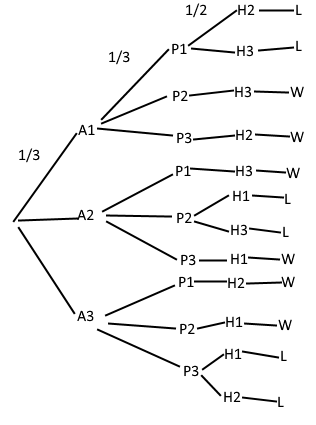
\includegraphics[width=\linewidth]{MontyHall.png}
\caption{Дерево вариантов}
\label{fig:MontyHall}
\end{figure}
Итак, сначала организаторы случайно (то есть, вероятность каждого из трех выборов - $\frac{1}{3}$) выбирают дверь, за которой помещают автомобиль (A1, A2, A3). Затем игрок делает свой выбор (P1, P2, P3), тоже случайно. Затем ведущий выбирает, какую дверь ему открыть. Заметим, что выбор у ведущего есть только если игрок исходно выбрал дверь, за которой находится приз. В таком случае, мы считаем, что ведущий делает выбор случайным образом (то есть, вероятность каждого из 2 выборов - $\frac{1}{2}$). Таким образом, мы получили набор элементарных исходов (листья дерева), каждый из которых имеет вид (Ax, Py, Hz) - выбор организаторов, выбор игрока, выбор ведущего. Вероятность каждого из таких исходов можно посчитать как произведение вероятностей на пути из корня дерева в лист, соответствующий данному исходу (то есть, $Pr(\{(A1, P1, H2)\}) = \frac{1}{3} * \frac{1}{3} * \frac{1}{2} = \frac{1}{18}$). Теперь нам нужно посчитать $Pr\{$Игрок выиграет, если сменит выбор$\}$. На картинке все исходы, удовлетворяющие этому условию, отмечены буквой W. Посчитав сумму их вероятностей, получим $\frac{2}{3}$.\\
Почему так получается? Очень грубо и не совсем корректно, зато интуитивно понятно, это можно объяснить так: вероятность того, что игрок исходно угадал - $\frac{1}{3}$. То есть с вероятностью $\frac{2}{3}$ автомобиль за одной из двух других дверей. Когда ведущий открывает дверь, мы не получаем никакой новой информации, т.к. заранее известно, что он должен был открыть дверь с козой. Значит, исходные $\frac{2}{3}$ вероятности, что игрок выбрал не ту дверь, остаются и сосредотачиваются на оставшейся двери, а значит, сменив выбор, игрок с вероятностью $\frac{2}{3}$ выиграет.\\
Еще до кучи всяких примеров с бросками монетки, бросками кубиков, вытягиванием карт, игрой в русскую рулетку и.т.д можно придумать и самим.
\subsubsection{Условная вероятность}
Пусть есть вероятностное пространство $(S, PR)$, $A, B \subseteq S$, $Pr(B) \not= 0$. Тогда вероятностью A при условии B (вероятность события A при условии, что известно, что событие B произошло) называют \\
$Pr(A|B) = \frac{Pr(A \cap B)}{Pr{B})}$.\\
\subsubsection{Задача о хоккейной команде}
ХК Локомотив играет серию до двух побед против СКА. Вероятность того, что Локомотив выиграет первую игру - $\frac{1}{2}$, а вот для остальных игр действует правило: если Локомотив выиграл предыдущую игру, вероятность его победы поднимается до $\frac{2}{3}$, а если проиграл - падает до $\frac{1}{4}$. Построим дерево возможных вариантов:\\
\begin{figure}
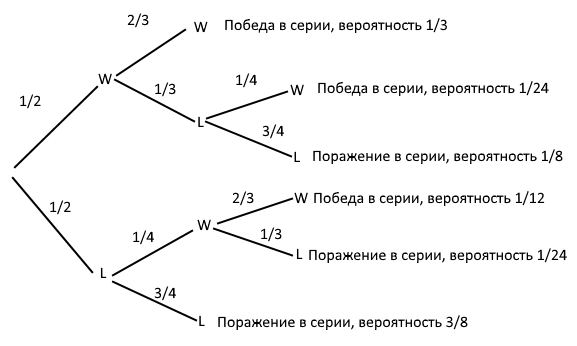
\includegraphics[width=\linewidth]{Hockey.png}
\caption{Дерево вариантов}
\label{fig:Hockey}
\end{figure}
Построим множество элементарных исходов $S = \{WW, WLW, WLL, LWW, LWL, LL\}$\\
Посчитаем несколько вероятностей:\\
\begin{itemize}
\item $Pr\{$Локомотив выиграет серию$\} = Pr(\{WW, WLW, LWW\}) = \frac{1}{3} + \frac{1}{24} + \frac{1}{12} = \frac{11}{24}$\\
\item $Pr\{$Локомотив выиграет серию, если он выиграл первую игру$\} = Pr(\{WW, WLW, LWW\}|\{WW, WLW, WLL\}) = \frac{Pr(\{WW, WLW\})}{Pr(\{WW, WLW, WLL\})} = \frac{\frac{1}{3} + \frac{1}{24}}{\frac{1}{2}} = \frac{3}{4}$\\
\item $Pr\{$Локомотив выиграл первую игру, если он выиграл серию$\} = Pr(\{WW, WLW, WLL\}|\{WW, WLW, LWW\}) = \frac{Pr(\{WW, WLW\})}{Pr(\{WW, WLW, LWW\})} = \frac{\frac{1}{3} + \frac{1}{24}}{\frac{1}{2}} = \frac{9}{11}$\\
\item $Pr\{$Локомотив выиграет вторую игру, если он выиграл первую игру$\} = Pr(\{WW, LWW, LWW\}|\{WW, WLW, WLL\}) = \frac{Pr(\{WW\})}{Pr(\{WW, WLW, WLL\})} = \frac{\frac{1}{3}}{\frac{1}{2}} = \frac{2}{3}$
\end{itemize}
\subsection{16.11.18}
(Большая часть этой лекции состояла из работы с задачей про хоккейную команду, что я включил в конспект прошлой лекции и из примера про вытаскивание шариков из урн, который мне разбирать лень. Так что всего один пункт. Всегда бы так, а.
\subsubsection{Свойства условной вероятности, формула Байеса}
\begin{itemize}
\item $Pr((A \cap B)|C) = Pr(A|(B \cap C)) * Pr(B|C)$. Доказывается проверкой по формуле условной вероятности.\\
\item Формула Байеса: $Pr(B|A) * Pr(A) = Pr(A \cap B) = Pr(A|B) * Pr(B)$. Доказывается проверкой по формуле условной вероятности.\\
\item $Pr(A_1 \cap \; ... \; \cap A_n) = Pr(A_1|(A_2 \cap \; ... \; \cap A_n)) * \; ... \; * Pr(A_{n - 1}|A_n) * Pr(A_n)$. Доказывается по индукции.\\
\end{itemize}

\subsection{23.11.18}
\subsubsection{Задача о медицинском обследовании}
Пусть существует некая болезнь "СПИД ноги", которой подвержены $10\%$ населения. \\
Есть тест на выявление этой болезни, который: \\
\begin{itemize}
\item Имеет $10\%$ вероятность ложного отрицания (вероятность отрицательного (N) результата теста, если человек болен (S)).\\
\item Имеет $30\%$ вероятность ложного подтверждения (вероятность положительного (P) результата теста, если человек здоров (H)).\\
\end{itemize}
Построим дерево вариантов:\\
\begin{figure}
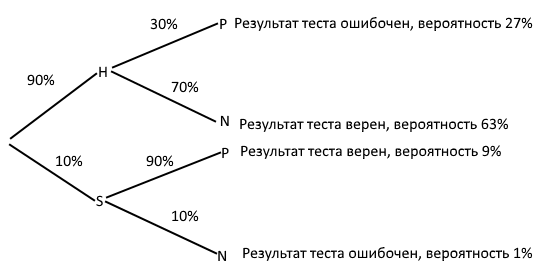
\includegraphics[width=\linewidth]{Medicare.png}
\caption{Дерево вариантов}
\label{fig:Medicare}
\end{figure}
Посчитаем несколько вероятностей:\\
\begin{itemize}
\item $Pr\{$Тест положительный$\} = Pr(\{HP, SP\}) = 9\% + 27\% = 36\%$. то есть, несмотря на то, что болеет всего $10\%$ населения, тест даст положительный результат более чем в $\frac{1}{3}$ случаев.\\
\item $Pr\{$Человек болен, если тест положительный$\} = Pr(\{SP, SN\}|\{HP, SP\}) = \frac{Pr(\{SP\})}{Pr(\{HP, SP\})} = \frac{9\%}{36\%} = 25\%$\\
\item $Pr\{$Тест работает верно$\} = Pr(\{HN, SP\}) = 63\% + 9\% = 72\%$
\end{itemize}
Кажется, что тест не очень эффективен. Но так ли это?\\
Рассмотрим инновационный тест (спонсированный военкоматом), который всегда выдает отрицательный результат.\\
Для такого чудесного теста $Pr\{$Тест работает верно$\} = Pr(\{HN, SP\}) = 90\% + 0\% = 90\%$.\\
Мораль: нужно аккуратно работать с вероятностями и не поддаваться на провокации.
\subsubsection{Задача об угадывании чисел в конвертах}
Итак, пусть есть два различных числа от 0 до 100 в закрытых конвертах. Вам предложено, открыв один из конвертов (наугад, то есть, конверты ничем не отличаются), попытаться угадать, открыли вы конверт с большим из двух чисел (H) или меньшим (L). Задача в том, чтобы научиться угадывать с вероятностью хотя бы чуть-чуть лучшей, чем $50\%$ при ЛЮБОЙ стратегии противника.\\
Давайте попробуем найти такое число X, что $L < X < H$. По имеющемуся X и числу из открытого конверта можно очень легко понять, какое из двух чисел меньше (если число из открытого конверта меньше X, то это L, иначе - H).\\
Чтобы избежать ситуаций, когда X совпадает с L или H, будем выбирать X из множества $A = \{\frac{1}{2}, \; ... \; , 99\frac{1}{2}\}$. Вопрос, собственно, в том, как выбрать хорошее число X?\\
Давайте попробуем просто наугад! Нарисуем дерево вариантов:\\
\begin{figure}
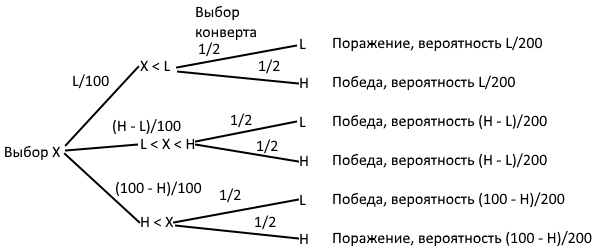
\includegraphics[width=\linewidth]{Envelopes.png}
\caption{Дерево вариантов}
\label{fig:Envelopes}
\end{figure}
Итак, посчитаем вероятность победы с использованием данной стратегии:\\
$Pr\{$победить$\} = \frac{L}{200} + \frac{H - L}{200} + \frac{H - L}{200} + \frac{100 - H}{200} = \frac{100 - H + H - L + L}{200} + \frac{H - L}{200} = \frac{1}{2} + \frac{H - L}{200}$,\\
то есть даже в худшем случае, когда противник выбрал два соседних числа, вероятность победить, используя данную стратегию составляет $50\frac{1}{2}\%$.
\subsubsection{Дискретная случайная величина}
Для вероятностного пространства $(S, Pr)$, $|S| < \infty$ функция $\xi: \; S \rightarrow \mathbb{R}$ называется дискретной случайной величиной (далее - ДСВ).\\
$Pr\{\xi = a\} = Pr(\{\omega \in S \; : \; \xi(\omega) = a\})$\\
$Pr\{\xi \leq a\} = Pr(\{\omega \in S \; : \; \xi(\omega) leq a\})$\\
Например для вероятностного пространства, иллюстрирующего три броска монетки, можно ввести дискретную случайную величину $\phi$, отражающую количество выпавших орлов. Тогда, например, $Pr\{\phi = 2\} = Pr(\{$РОО,ОРО,ООР$\}) = \frac{3}{8}$
\subsubsection{Математическое ожидание ДСВ}
Математическим ожиданием (матожиданием) ДСВ $\xi$ на вероятностном пространстве $(S, Pr)$ называют\\
$E \xi = \sum\limits_{\omega \in S}\xi(\omega) * Pr(\{\omega\})$\\
Альтернативная формула матожидания:\\
$E \xi = \sum\limits_{a \in Im(\xi)} \sum_{\omega \in S, \xi(\omega) = a} a * Pr(\{\omega\}) = \sum\limits_{a \in Im(\xi)} a * \sum_{\omega \in S, \xi(\omega) = a}Pr(\{\omega\}) = \sum\limits_{a \in Im(\xi)} a * Pr(\{\omega \in S \; : \; \xi(\omega) = a\}) = \sum\limits_{a \in Im(\xi)} a * Pr\{\xi = a\}$\\
Также можно заметить, что если изобразить числовую прямую как балку, и на каждой точке a из $Im(\xi)$ нарисовать столбик высоты $Pr\{\xi = a\}$, матожидание $\xi$ будет лежать на числовой прямой в той точке, на которой эту балку можно сбалансировать.\\
Вот рисунок для матожидания количества орлов, выпавших после броска трех монет:\\
\begin{figure}
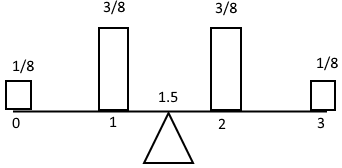
\includegraphics[width=\linewidth]{HeadsTails.png}
\caption{Матожидание количества орлов}
\label{fig:HeadsTails}
\end{figure}
\subsubsection{Арифметические действия с ДСВ и матожиданием}
\begin{itemize}
\item $\eta = \xi + c$ определим как $\eta(\omega) = \xi(\omega) + c$. $Pr\{\eta = a\} = Pr\{\xi + c = a\} = Pr\{\xi = a - c\}$. По второй формуле матожидания можно заметить, что $E \eta = c + E \xi$\\
\item $\eta = \xi * c$, $c \not= 0$ определим как $\eta(\omega) = \xi(\omega) * c$. $Pr\{\eta = a\} = Pr\{\xi * c = a\} = Pr\{\xi = \frac{a}{c}\}$. По второй формуле матожидания можно заметить, что $E \eta = c * E \xi$\\
\item $\eta = \xi^2$ определим как $\eta(\omega) = (\xi(\omega))^2$. $Pr\{\eta = a\} = Pr\{\xi^2 = a\}$. $E \eta = \sum\limits_{\omega \in S}\xi^2(\omega) * Pr(\{\omega\})$\\
\item $\eta = \xi + \psi$ определим как $(\xi + \psi)(\omega) = \xi(\omega) + \psi(\omega)$. $E (\\xi + \psi) = \sum\limits_{\omega \in S} (\xi(\omega) + \psi(\omega)) * Pr(\{\omega\}) = \sum\limits_{\omega \in S} \xi(\omega) * Pr(\{\omega\}) + \sum\limits_{\omega \in S} \psi(\omega) * Pr(\{\omega\}) = E \xi + E \psi$
\end{itemize}
\subsubsection{Дисперсия ДСВ}
Дисперсией ДСВ называют матожидание квадрата разности значения ДСВ и ее матожидания:\\
$D \xi = E (\xi - E \xi)^2$.\\
$E (\xi - E \xi)^2 = E (\xi^2 - 2 * E \xi * \xi + (E \xi)^2) = E \xi^2 - E (2 * E \xi * \xi)) + E (E \xi)^2 = E \xi^2 - 2 * E \xi * E \xi + (E \xi)^2 = E \xi^2 - (E \xi)^2$\\
Таким образом, $D \xi = E \xi^2 - (E \xi)^2$.
\subsection{30.11.18}
\subsubsection{Испытание Бернулли}
Пусть на произвольном вероятностном пространстве $(S, Pr)$ объявлена ДСВ $\xi$ такая, что $Pr\{\xi = 1\} = p, Pr\{\xi = 0\} = 1 - p$. Словами это можно обосновать так: каждый элементарный исход $\omega \in S$ считается либо успешным ($\xi(\omega) = 1$), либо неудачным ($\xi(\omega) = 0$). Тогда:\\
$E \xi = 0 * (1 - p) + 1 * p = p$\\
$D \xi = E \xi^2 - (E \xi)^2 = (1 - p) * 0^2 + p * 1^2 - p^2 = p - p^2 = p(1 - p)$
\subsubsection{Моделирование ДСВ, генераторы случайных чисел}
Многократно повторяемый эксперимент, исходы которого имеют заданный набор вероятностей, соответствующий набору вероятностей ДСВ, называют моделью этой ДСВ.\\
Пример: моделью $\xi$ ($Pr\{\xi = 0\} = \frac{1}{2}, Pr\{\xi = 1\} = \frac{1}{2}$) можно считать бросок монетки (если считать, что стороны монетки одинаковые, монетка никогда не падает на ребро и бросают ее наугад).\\
Многократно повторяемый эксперимент, результатом которого является (псевдо)случайно выбранное число из некоторого конечного множества, называют дискретным генератором (датчиком) случайных чисел.\\
Пример: назовем $\alpha$ дискретный генератор случайных чисел, для которого $Pr\{\alpha = k\} = \frac{1}{N} \; \forall k \in 1:N$.\\
Многократно повторяемый эксперимент, результатом которого является (псевдо)случайно выбранное число из некоторого промежутка числовой прямой, называют непрерывным генератором (датчиком) случайных чисел.\\
Пример: назовем $\alpha_0$ непрерывный генератор случайных чисел, который с равной вероятностью попадает в каждую из точек отрезка $[0, 1]$.\\
Поскольку отрезок $[0, 1]$ содержит несчетное количество точек, вероятность $Pr\{\alpha_0 = x\} = \frac{1}{\infty} = 0 \; \forall x \in [0, 1]$. Однако, вероятность того, что точка попадет в некоторый промежуток, все же ненулевая:\\
$Pr\{x \in <a, b>\} = \frac{|<a, a + \delta>|}{|[0, 1]|} = \frac{\delta}{1} = \delta$\\
В частности, $Pr\{x \in [0, 1]\} = 1$.\\
Замечание: поскольку для конкретной точки вероятность попадания туда $\alpha_0$ равна нулю, можно смело выкидывать из множества конечное (и даже счетное) количество точек, и вероятность попадания в него останется неизменной. Следовательно, вместо $<a, b>$ можно рассматривать $(a, b)$ или $[a, b)$. Последнее особенно удобно, поскольку полуинтервалы хорошо стыкуются.
\subsubsection{Табличный метод моделирования ДСВ}
Итак, пусть есть вероятностное пространство $(S, Pr)$ и заданная на нем ДСВ $\xi$.\\
При этом $S = \{0, 1, \; ... \; , n - 1\}$, $\forall i \in 0:(n - 1) \; Pr(\{i\}) = p_i$, $\sum\limits_{i = 0}^{n - 1} p_i = 1$.\\
Примечание: для ДСВ с произвольным набором значений можно их пронумеровать и свести задачу к данной.
Возьмем отрезок $[0, 1)$ и поделим его на полуинтервалы вида $[x_i, x_{i + 1})$, где $x_0 = 0$, $\forall i \in 0:(n - 1) \; x_{i + 1} = x_i + p_i$\\
Для такого разбиения отрезка $[0, 1]$ вероятность $Pr\{\alpha_0 \in [x_i, x_{i + 1}]\} = p_i$. То есть, эксперимент "в отрезок с каким номером попадет случайное число, выданное $\alpha_0$?" моделирует $\xi$.\\
Замечание: При попадании в точку 1 значение $\alpha_0$ оказывается вне пределов всех полуинтервалов. Но с одной стороны, вероятность такого события - 0, так что распределение вероятностей это нам не портит, а с другой, если это все же произошло, мы можем просто объявить эксперимент неудачным и провести его заново.\\
Основным недостатком данного метода является большое количество сравнений вещественных чисел, каковая операция является не очень точной и достаточно долгой. Неплохо бы придумать метод, который минимизирует количество таких операций.
\subsubsection{Метод Уокера}
В табличном методе мы располагали полуинтервалы на отрезке $[0, 1]$ в произвольном порядке. В этот раз мы сначала разделим его на полуинтервалы $[\frac{i}{n}, \frac{i + 1}{n}) \; \forall i \in 0:(n - 1)$ (назовем их базовыми полуинтервалами. Такого обозначения на лекции не было, но я не хочу каждый раз уточнять, имею я в виду эти полуинтервалы или те, длины которых равны вероятностям) и будем следить, чтобы в одном таком полуинтервале было не более одной границы полуинтервалов, соответствующих исходам. Более того, если раньше каждому исходу соответствовал ровно один полуинтервал, то сейчас их может быть несколько, главное только, чтобы сумма их длин все еще была равна вероятности этого исхода.\\
Зачем? Давайте посмотрим на число $n * \alpha_0$. \\
Утверждение: его целая часть $\lfloor n * \alpha_0 \rfloor$ будет равно i, если $\frac{i}{n} \leq \alpha_0 < \frac{i + 1}{n}$.\\
Доказательство: умножим все части неравенства на n: $i \leq n * \alpha_0 < i + 1 \Leftrightarrow \lfloor n * \alpha_0 \rfloor = i$.\\
Итак, мы научились понимать, в какой базовый полуинтервал попал $\alpha_0$. Теперь осталось понять, что делать, если в базовом полуинтервале есть граница между полуинтервалами. Пусть эта граница есть в точке $x, \frac{i}{n} \leq x < \frac{i + 1}{n}$. Растянем наш базовый полуинтервал в n раз:\\
Точка $\frac{i}{n}$ перейдет в точку $i = \lfloor n * \alpha_0 \rfloor$, $\alpha_0$ - в $n * \alpha_0$, x - в $n * x$, $\frac{i + 1}{n}$ - в $i + 1 = \lfloor n * \alpha_0 \rfloor + 1$.\\
Теперь сдвинем полуинтервал влево на i: $\lfloor n * \alpha_0 \rfloor$ перейдет в 0, $n * \alpha_0$ - в $\{n * \alpha_0\}$ (дробная часть), $n * x$ - в $n * x - i$, $\lfloor n * \alpha_0 \rfloor + 1$ - в 1. То есть, теперь нам достаточно сравнить $\{n * \alpha_0\}$ и $n * x - i$, причем $n * x - i$ не зависит от $\alpha_0$ и может быть посчитана заранее.\\
Замечание: при попадании в единицу нам все еще придется повторять опыт.\\
Итак, пусть каждому значению случайной величины $i \in 0:(n - 1)$ соответствует множество $P_i$ полуинтервалов, причем каждый из них полностью лежит в одном из базовых полуинтервалов и пересечение $P_i$ и $P_j$ пусто для любого $j \not= i$, а $\sum\limits_{[a, b) \in P_i}|[a, b)| = p_i$. Также, в каждом базовом полуинтервале лежит не более двух полуинтервалов.\\
Тогда мы научились с помощью двух сравнений понимать, в какой полуинтервал $[a, b)$ попал $\alpha_0$, а если объявить исходом эксперимента i, где $[a, b) \in P_i$, то этот эксперимент будет моделировать $\xi$, так как вероятность попасть в полуинтервал, лежащий в $P_i$ равна $\sum\limits_{[a, b) \in P_i}Pr\{\alpha_0 \in [a, b)\} = \sum\limits_{[a, b) \in P_i}|[a, b)| = p_i$ Осталось только построить такое разбиение.\\
Для этого нам придется доказать две леммы:\\
Лемма 1: если $n > 1$, $\exists l \in 0:(n - 1): \; p_l \leq \frac{1}{n}$. Доказательство: если нет, то $\sum\limits_{i = 0}^{n - 1} p_i > 1$.\\
Лемма 2: если $n > 1$, $\forall l \in 0:(n - 1) \; \exists m \in 0:(n - 1), m \not= l : \; p_l + p_m > \frac{1}{n}$. Доказательство: если нет, то $\exists l_0 \in 0:(n - 1)$ такое, что:\\
$\sum\limits_{m \not= l_0} (p_{l_0} + p_m) \leq \frac{n - 1}{n} < 1$\\
С другой стороны, $\sum\limits_{m \not= l_0} (p_{l_0} + p_m) = \sum\limits_{m \not= l_0} p_{l_0} + \sum\limits_{m \not= l_0}p_m = (n - 1) * p_{l_0} + \sum\limits_{m \in 0:(n - 1)}p_m \geq 1$. Противоречие.\\
Итак, начнем строить наше разбиение:\\
Определим $\xi^{(0)}: p^{(0)}_i = p_i$, выберем $l_0: \; p^{(0)}_{l_0} < \frac{1}{n}$, $m_0: \; p^{(0)}_{l_0} + p^{(0)}_{m_0} > \frac{1}{n}$\\
Определим ДСВ $\psi^{(0)}: \; Pr\{\psi^{(0)} = l_0\} = n * p^{(0)}_{l_0}\}, Pr\{\psi^{(0)} = m_0\} = 1 - n * p^{(0)}_{l_0}\}$.\\
Теперь отрежем от отрезка $[0, 1]$ первый базовый полуинтервал:\\
$\xi^{(1)}: p^{(1)}_{l_0} = 0, p^{(1)}_{m_0} = (p^{(0)}_{m_0} - (\frac{1}{n} - p^{(0)}_{l_0})) * \frac{n}{n - 1},  p^{(1)}_i = p_i * \frac{n}{n - 1}$ и перейдем к следующему шагу алгоритма.\\
Теперь научимся вычислять $\forall k \in 0:(n - 1) \; p^{(0)}_i$ через $\xi^{(1)}$:\\
$p^{(0)}_k = \frac{1}{n}Pr\{\psi^{(0)} = k\} + \frac{n - 1}{n}p^{(1)}_k$\\
Корректность этой формулы можно аккуратно руками проверить.\\
Теперь рассмотрим общий случай:\\
Пусть построено $\xi^{(i)}$, $i \geq 1$, у этой ДСВ $n - i$ возможных исходов.\\
$\exists l_i, m_i: \; m_i \not= l_i, p^{(i)}_{l_i} \leq \frac{1}{n - i}, p^{(i)}_{m_i} + p^{(i)}_{l_i} > \frac{1}{n - i}$.\\
$\psi^{(i)}: \; Pr\{\psi^{(i)} = l_i\} = (n - i) * p^{(i)}_{l_0}, Pr\{\psi^{(i)} = m_i\} = 1 - (n - i) * p^{(i)}_{l_0}$\\
Строим $\xi^{(i + 1)}$: $p^{(i + 1)}_{l_i} = 0, p^{(i + 1)}_{m_i} = p^{(i)}_{m_i} - \frac{n - i}{n - i - 1}(\frac{1}{n - i} - p^{(i)}_{l_i}), p^{(i + 1)}_{s} = \frac{n - i}{n - i - 1}p^{(i)}_{s}$\\
Тогда $p^{(i)}_{k} = \frac{1}{n - i}Pr\{\psi^{(i)} = k\} + \frac{n - i - 1}{n - i}p^{(i + 1)}_{k}$.\\
Так до $n - 1$ шага. На $n - 1$ шаге получаем, что $\xi^{(n - 1)}$ имеет всего один возможный исход: $Pr\{\xi^{(n - 1)} = l_{n - 1}\} = 1$. \\
Тогда $p^{(n - 1)}_k = \frac{1}{1}Pr\{\psi^{(n - 1)} = k\} + 0 = Pr\{\psi^{(n - 1)} = k\}$.\\
Таким образом, мы получили рекурсивную формулу для $p^{(i)}_k$. Раскроем ее:\\
$p_k = p^{(0)}_k = \frac{1}{n}Pr\{\psi^{(0)} = k\} + \frac{n - 1}{n}p^{(1)}_k = \frac{1}{n}Pr\{\psi^{(0)} = k\} + \frac{n - 1}{n}(\frac{1}{n - 1}Pr\{\psi^{(1)} = k\} + \frac{n - 2}{n - 1}p^{(2)}_k) = \frac{1}{n}Pr\{\psi^{(0)} = k\} + \frac{1}{n}Pr\{\psi^{(1)} = k\} + \frac{n - 2}{n}p^{(2)}_k = ... = \frac{1}{n}\sum\limits_{j \in 0:(n - 1)}Pr\{\psi^{(j)} = k\}$\\.
Пример: $p_0 = 0.91, p_1 = p_2 = p_3 = p_4 = p_5 = p_6 = p_7 = p_8 = p_9 = 0.01$.\\
На первом шаге $l_0 = 1, m_0 = 0$. Тогда $p^{(1)}_1 = 0$, $p^{(1)}_0 = \frac{10}{9}(p^{(0)}_0 - (\frac{1}{10} - p^{(0)}_0)) = \frac{10}{9}(p_0 - \frac{1}{10} + p_1) = \frac{10}{9}(0.91 - 0.1 + 0.01) = \frac{10}{9}0.82$, $p^{(1)}_i = \frac{10}{9}(p^{(0)}_i) = \frac{0.1}{9}$.\\
И так далее, на последнем шаге получим $p^{(9)}_0 = 1$, $p^{(9)}_i = 0$.\\
\begin{figure}[H]
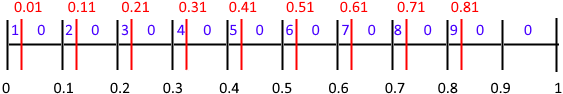
\includegraphics[width=\linewidth]{Walker.png}
\caption{Разбиение}
\label{fig:Walker}
\end{figure}
На рисунке черным обозначены границы базовых полуинтервалов, красным - границы полуинтервалов, синим - номера исходов, соответствующих данным полуинтервалам.
\subsection{07.12.18}
\subsubsection{Вычислительная схема метода Уокера}
Заметим, что постоянное домножение на коэффициенты в методе Уокера нужно только чтобы на каждом шаге $\xi^{(i)}$ оставалась ДСВ, что необходимо для формального доказательства, но совершенно не нужно для практических вычислений.\\
В приведенной ниже таблице коэффициенты вынесены за скобки (самый левый столбец), и по большей части игнорируются.\\
\begin{figure}[H]
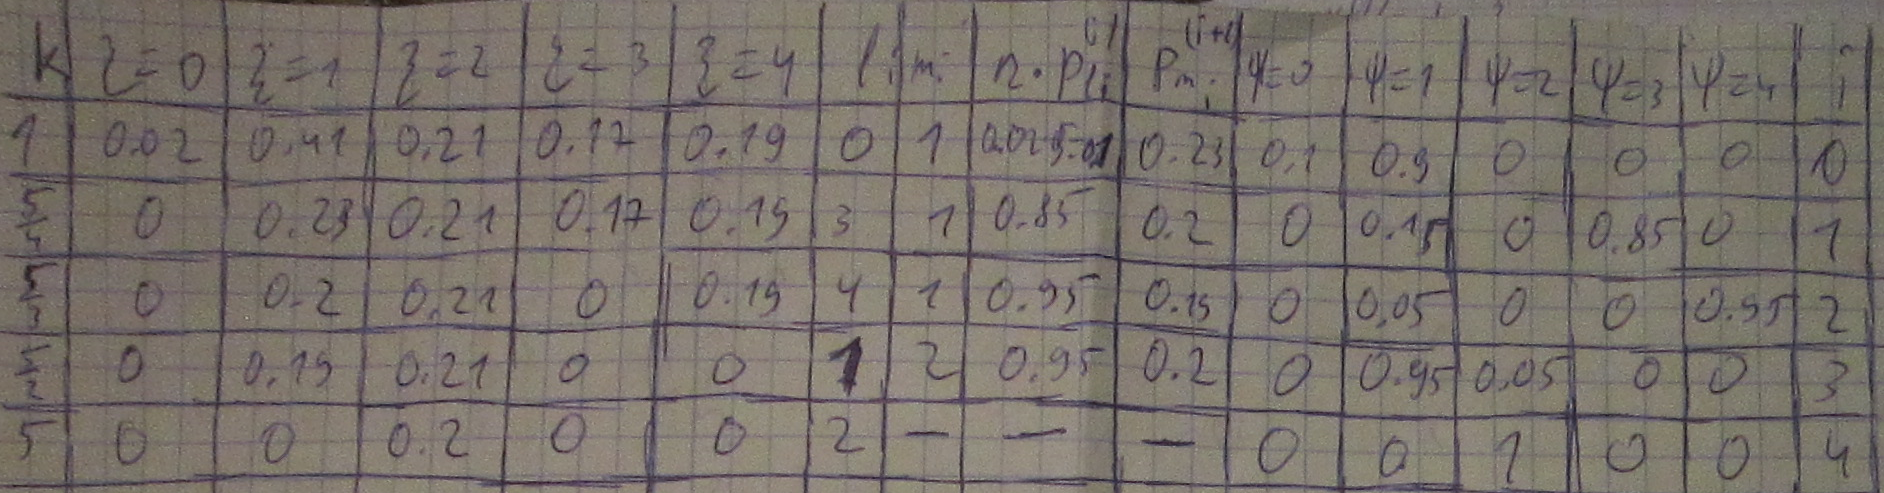
\includegraphics[width=\linewidth]{WalkerTable.png}
\caption{Вычислительная схема}
\label{fig:WalkerTable}
\end{figure}
Следующие 5 столбцов показывают набор вероятностей для $\xi^{(i)}$, затем идут номер $l_i$, номер $m_i$, значение $n * p^{(i)}_{l_i}$, необходимое для построения $\psi^{(i)}$, значение $p^{(i + 1)}_{m_i} = p^{(i)}_{m_i} - \frac{1}{n} + p^{(i)}_{l_i}$ (без домножения на коэффициент!), необходимое для пересчета $\xi^{(i + 1)}$, затем набор вероятностей $\psi^{(i)}$, ну и наконец само i. Здесь стоит заметить, что i - это не только номер текущего шага алгоритма, но и номер базового полуинтервала, который мы на этом шаге алгоритма делим.\\
Как же пользоваться этой схемой? Рассмотрим на примере:\\
Пусть $\alpha_0 = 0.73$. Тогда $n * \alpha_0 = 5 * 0.73 = 3.65$. $\lfloor n * \alpha_0 \rfloor = 3$, значит, мы попали в третий базовый полуинтервал. Граница между полуинтервалами в нем проходит по $n * p^{(i)}_{l_i} = 5 * p^{(3)}_{l_3} = 0.95$. Дробная часть  $\{n * \alpha_0\} = 0.65 < 0.95$, значит, результат эксперимента - $l_i = l_3 = 1$.
\subsubsection{Моделирование ДСВ с помощью последовательности (псевдо)случайных бит.}
Псевдослучайный бит - 0 или 1 равновероятно (бросок монетки).\\
Чего мы хотим? Научиться моделировать ДСВ, вероятности которой - рациональные двоичные числа, с помощью последовательности случайных бит.\\
Пример: $\xi: \; Pr\{\xi = 0\} = \frac{1}{4} = 0.01_2, Pr\{\xi = 1\} = \frac{1}{2} = 0.1_2, Pr\{\xi = 2\} = \frac{1}{4} = 0.01_2$\\
Казалось бы, можно построить полное двоичное дерево нужной глубины h (равной максимальному количеству значащих двоичных цифр после запятой среди $p_i$) и каким-то образом распределить листья по исходам так, чтобы количество листьев, соответствующих i-му исходу было равно $2^h * p_i$. Однако, посмотрим на два различных корректных способа распределения листьев между исходами:\\
\begin{figure}[H]
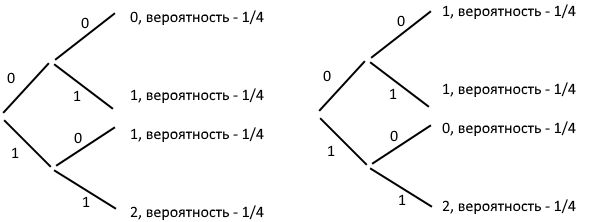
\includegraphics[width=\linewidth]{Bits1.png}
\caption{Сравнение способов}
\label{fig:Bits1}
\end{figure}
В первом случае нам в любом случае придется бросать монетку дважды, а вот во втором если первый бросок монетки выдал результат 0, дальше можно уже не бросать - нам точно известно, что результатом эксперимента будет 1.\\
Собственно, задача изложенного ниже алгоритма в том, чтобы минимизировать среднее число бросков монетки, необходимое для получения результата. Такое разбиение множества листьев будем называть оптимальным.\\
Формализуем:\\
Пусть есть ДСВ $\xi$, $\forall i \in 0:(n - 1) \; Pr\{\xi = i\} = p_i$, $\sum\limits_{i \in 0:(n - 1)}p_i = 1$.\\
$p_i$ в двоичной записи имеет представление $0.\pi^i_1\pi^i_2...\pi^i_m$, то есть $p_i = \frac{\pi^i_1}{2} + \frac{\pi^i_2}{4} + ... + \frac{\pi^i_m}{2^m}$, где $\pi^i_k \in \{0, 1\}$. Тогда $2^mp_i = 2^{m - 1}\pi^i_1 + ... + \pi^i_{m}$.\\
Рассмотрим множество A исходов m бросков монетки. $|A| = 2^m$.\\
Рассмотрим разбиение $A = A_0 \cup A_1 \cup ... \cup A_{n - 1}$, где $\forall i \in 0:(n - 1) \; |A_i| = 2^mp_i$.\\
Тогда если исход эксперимента "m бросков монетки" лежит в $A_i$, то регистрируем исход i. $Pr\{$зарегистрирован исход i$\} = \frac{|A_i|}{2^m} = p_i$. Но как построить оптимальное разбиение?\\
Заведем набор множеств $\forall k \in 1:m \; I_k = \{i \in 0:(n - 1) \; : \; \pi^i_k = 1\}$.\\
Пусть мы бросили монету 1 раз. Множество исходов $B_1$ имеет мощность 2. Выберем какое-то $M_1 \subseteq B_1$ такое, что $|M_1| = |I_1| = \sum\limits_{j \in 0:(n - 1)}\pi^j_1$. Установим биекцию между $M_1$ и $I_1$. Во всех этих случаях исход уже определен, а в остальных $B_1 \setminus M_1$ случаях нам нужно продолжать бросать.\\
Теперь у нас есть $B_2, |B_2| = 2|B_1 \setminus M_1|$, продолжаем использовать тот же алгоритм.\\
В общем случае, у нас есть $B_k$ - множество исходов после k бросков монетки, выбираем из них множество $M_k \subseteq B_k$ исходов такое, что $|M_k| = |I_k|$, строим биекцию между $M_k$ и $I_k$, определяя исход эксперимента для этих случаев, а в остальных $B_k \setminus M_k$ случаях продолжаем бросать.\\
Пример:\\
$p_0 = 0.101001; p_1 = 0.000001; p_2 = 001101; p_3 = 001001$. Тогда:\\
$I_0 = \{0\}$\\
$I_1 = \varnothing$\\
$I_2 = \{0, 2, 3\}$\\
$I_3 = \{2\}$\\
$I_4 = \varnothing$\\
$I_5 = \{0, 1, 2, 3\}$\\
\begin{figure}[H]
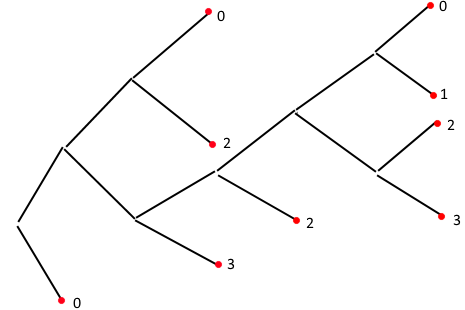
\includegraphics[width=\linewidth]{Bits2.png}
\caption{Дерево вариантов}
\label{fig:Bits2}
\end{figure}
Таким образом, матожидание числа бросков равно:\\
$E\{$число бросков$\} = \sum\limits_{k \in 1:m}k * Pr\{$монета брошена k раз$\} = \sum\limits_{k \in 1:m}k|I_k|\frac{1}{2^k} = \sum\limits_{k \in 1:m}\frac{k}{2^k}\sum\limits_{j \in 0:(n - 1)}\pi^j_k$.
 
\subsection{08.12.18}
\subsubsection{Префиксный код}
$\Lambda$ - произвольное конечное множество (алфавит). $a \in \Lambda$ - символы.\\
$\forall a \in \Lambda \; \exists l(a) \in \mathbb{N}, \exists c(a) = \{0, 1\}^{l(a)}$ - кодовая последовательность a.\\
$\forall a, b \in \Lambda, a \not= b \; c(a) \not= c(b)$. Казалось бы, это достаточное условие, чтобы по коду однозначно распознавался символ. Но рассмотрим случай:\\
$\Lambda = \{a, b\}$, $c(a) = 10$, $c(b) = 100$. Тогда последовательность $100$ получатель сообщения может начать распознавать как "a???", а поскольку 0 не является валидным кодом, получатель не сможет расшифровать сообщение без каких-то дополнительных усилий. Если же добавить в алфавит символы $d, c(d) = 01$ и $e, c(e) = 1$, сообщение $1001$ можно будет понять и как $aв$, и как $be$.\\
Чтобы избежать подобных проблем, вводят условие префиксности:\\
Код называется префиксным, если $\forall a, b \in \Lambda \; c(a) = w \Rightarrow \not\exists m \in \mathbb{N}_0: \; c(b) = w\gamma$, где $\gamma \in \{0, 1\}^m$.\\
Иначе говоря, код называется префиксным, если никакая кодовая последовательность одного символа не является началом кодовой последовательности другого символа. Заметим также, что данное условие включает в себя условие несовпадения кодов различных символов, так что в дальнейшем отдельно рассматривать мы его не будем.\\
\subsubsection{Задача об оптимальном префиксном коде}
Пусть каждому символу $a \in \Lambda$ соответствует $p(a)$ - вероятность появления этого символа в сообщении. (Поскольку сообщение состоит из одного символа, $\sum\limits_{a \in \Lambda}p(a) = 1$. Также считаем, что $\forall a \in \Lambda \; p(a) > 0$).\\
Введем ДСВ $l: \; \forall a \in \Lambda \; Pr\{l = l(a)\} = p(a)$ - длина кодовой последовательности символа в сообщении.\\
Оптимальным называется префиксный код, минимизирующий матожидание l: $E \: l = \sum\limits_{a \in \Lambda}l(a)p(a)$\\
Интуитивно понятно, что чем чаще встречается символ, тем короче должна быть его кодовая последовательность. Но вот как это формализовать?\\
Договоримся про обозначения: здесь и далее считаем, что символы с одинаковыми прибамбасами (волна, палочка, штрих, два штриха и.т.д) относятся к коду с таким же прибамбасом, обговаривать это каждый раз не будем. То есть, $C' = \{(a, l'(a), c'(a)) \; : \; a \in \Lambda\}$, например.\\
Существование оптимального префиксного кода: ну, мы знаем, что $E \: l \geq 1$, ведь в каждой кодовой последовательности должен быть хотя бы один символ. Ну и мы знаем, что в худшем случае мы можем сделать префиксный код, в котором все символы имеют одинаковые длины кодовых последовательностей и эти последовательности различны. В таком случае $\forall a \in \Lambda \; l(a) = \lceil \log_2(|\Lambda|)$, так что префиксные коды существуют и матожидание длины кодовой последовательности ограничено.\\
Лемма 1: Если в некотором (не обязательно оптимальном) коде C существует $x \in \Lambda: \; c(x) = w\alpha$, где $\alpha \in \{0, 1\}$, и при этом $\not\exists y \in \Lambda, y \not= x: \; c(y) = w\gamma$, где $\gamma \in \{0, 1\}^k$ (то есть, если w не является началом никакой другой кодовой последовательности, кроме $c(x)$), то код $C'$ такой, что $c'(x) = w, \forall y \in \Lambda, y \not= x \; c'(y) = c(y)$ во-первых будет префиксным (по построению, префиксности C и условию леммы), а во-вторых, $E \: l' = E \: l - p(x)l(x) + p(x)(l(x) - 1) = E \: l - p(x) < E \: l$.\\
Тогда получается, что код C точно не мог быть оптимальным.\\
Лемма (*), которой не было в лекции, но она удобная: если в префиксном коде C $\exists a, b \in \Lambda, a \not= b: \;p(a) < p(b), l(a) < l(b)$, то такой код не оптимален. Доказательство: проверим, что для кода $C'$, в котором $c'(a) = c(b), c'(b) = c(a), \forall x \in \Lambda, x \not= a, x \not= b \; c'(x) = c(x)$\\
$E \: l - E \: l' = p(a)l(a) + p(b)l(b) - p(a)l(b) - p(b)l(a) = p(a)(l(a) - l(b)) - p(b)(l(a) - l(b)) = (p(a) - p(b))(l(a) - l(b)) > 0$.\\
Лемма 2: Пусть $a, b \in \Lambda, a \not= b$ - два символа с наименьшими вероятностями (для определенности, $\forall x \in \Lambda \; p(x) \leq p(b) \leq p(a)$). Тогда существует оптимальный префиксный код такой, что в нем $c(a) = w0, c(b) = w1$, где $\exists k \in \mathbb{N}_0: \; w \in \{0, 1\}^k$, и это самые длинные кодовые последовательности.\\
Доказательство: пусть $C'$ - какой-то оптимальный префиксный код. По лемме (*) a и b имеют самые длинные кодовые последовательности в $C'$: $\forall x \in \Lambda, x \not= a, x \not= b \; l'(a) \geq l'(b) \geq l'(x)$. Если $c(a) = w\gamma, w \in \{0, 1\}^{l(b)}, \gamma \in \{0, 1\}^{l(a) - l(b)}$ и w не является началом никакой кодовой последовательности (а он не является, т.к. все остальные кодовые последовательности не длиннее w, и при этом никакой символ не может иметь кодовую последовательность w, так как тогда нарушалась бы префиксность $C'$), то можно сократить кодовую последовательность a, создав более оптимальный код, что противоречит оптимальности $C'$.\\
Таким образом, мы узнали, что поскольку $C'$ оптимален, $l(a) = l(b)$. Ну а теперь дело техники: пусть $c'(b) = w1$ (если заканчивается на ноль, делаем все аналогично и в конце меняем коды местами), тогда если $\exists x \in \Lambda: \; c'(x) = w0$, построим оптимальный (поскольку длины кодовых последовательностей не изменились) код С: $c(a) = c'(x), c(x) = c'(a), \forall z \in \Lambda, z \not= a, z \not= x \; c(z) = c'(z)$. Если же такого x не нашлось, то построим оптимальный (поскольку длины кодовых последовательностей не изменились) код С: $c(a) = w0, \forall z \in \Lambda, z \not= a \; c(z) = c'(z)$. Лемма доказана.\\
Лемма 3: $\forall x \in \Lambda, x \not= a, x \not= b \; p(a) \leq p(b) \leq p(x)$.\\
$\Lambda' = \Lambda \setminus \{a, b\} \cup \{\underbrace{ab}\}$, где $\underbrace{ab} \not\in \Lambda, p(\underbrace{ab}) = p(a) + p(b)$.\\
Пусть $C'$ - оптимальный префиксный код для $\Lambda'$, $c'(\underbrace{ab}) = w$. Тогда для $\Lambda$ код С:\\
$c(a) = w0, c(b) = w1, \forall x \in \Lambda, x \not= a, x \not= b \; c(x) = c'(x)$ будет оптимальным префиксным кодом.\\
Доказательство: $l(a)p(a) + l(b)p(b) = (l'(\underbrace{ab}) + 1)(p(a) + p(b)) = l'(\underbrace{ab})p(\underbrace{ab}) + p(\underbrace{ab})$ Тогда $E \: l = E \: l' + p(\underbrace{ab})$.\\
Пусть $\overline{C}$ - оптимальный код для $\Lambda$, причем $E \: \overline{l} < E \: l$.\\
По лемме 2: $\overline{c}(a) = \gamma0, \overline{c}(b) = \gamma1$.\\
Построим $\overline{C}'$ для $\Lambda'$: $\overline{c}'(\underbrace{ab}) = \gamma, \forall x \in \Lambda, x \not= a, x \not= b \; \overline{c}'(x) = \overline{c}(x)$\\
Является ли $\overline{С}'$ префиксным кодом? Да. Никакой символ по лемме (*) не мог иметь кодовую последовательность длины $> \overline{l}(a)$. Никакой символ не мог иметь кодовую последовательность w, так как $\overline{C}$ префиксный. А единственные две последовательности длины $\overline{l}(a)$, начинающиеся на w, - это коды символов a и b, которых в $\Lambda'$ нет. \\
При этом, $E \: \overline{l} = E \: \overline{l}' + p(\underbrace{ab})$. Но поскольку по предположению $E \: l = E \: l' + p(\underbrace{ab}) > E \: \overline{l} = E \: \overline{l}' + p(\underbrace{ab})$, получаем $E \: l' > E \: \overline{l}'$, что противоречит оптимальности $C'$ на $\Lambda'$.\\
Значит, предположение неверно и $E \: \overline{l} \geq E \: l$, но так как $\overline{C}$ оптимален, $E \: \overline{l} = E \: l$, то есть C оптимален. Лемма доказана.
\subsubsection{Алгоритм Хаффмана построения оптимального префиксного кода.}
Итак, нам нужно построить оптимальный префиксный код на алфавите $\Lambda$, $|\Lambda| = M$.\\
Возьмем $\Lambda_0 = \Lambda$.\\
$\forall k \in 0:(M - 3)$ возьмем $a_k, b_k \in \Lambda_k$ такие, что $\forall x \in \Lambda_k, x \not= a_k, x \not= b_k \; p_k(a_k) \leq p_k(b_k) \leq p_k(x)$ и построим $\Lambda_{k + 1} = \Lambda_{k} \setminus \{a_k, b_k\} \cup \{\underbrace{a_kb_k}\}$.\\
Для $\Lambda_{M - 2} = \{a_{M - 2}, b_{M - 2}\}$ оптимальным, очевидно, будет код $C_{M - 2}: \; c_{M - 2}(a_{M - 2}) = 0, c_{M - 2}(b_{M - 2}) = 1$, так как для него $E \: l_{M - 2} = 1$.\\
Теперь пусть для $k \in 1:(M - 2)$ у нас есть оптимальный префиксный код $C_k$ для $\Lambda_k$. По лемме 3 построим оптимальный префиксный код $C_{k - 1}$ для $\Lambda_{k - 1}$: $c_{k - 1}(a_{k - 1}) = c_k(\underbrace{a_{k - 1}b_{k - 1}})0, c_{k - 1}(b_{k - 1}) = c_k(\underbrace{a_{k - 1}b_{k - 1}})1, \forall x \in \Lambda_k, x \not= \underbrace{a_{k - 1}b_{k - 1}} \; c_{k - 1}(x) = c_k(x)$\\
Так строим, пока не получим $C_0$ - оптимальный префиксный код для $\Lambda_0 = \Lambda$.\\
Пример:\\
$\Lambda = \{a, b, c, d, e, f, g\}$, $p(a) = 0.13, p(b) = 0.08, p(c) = 0.25, p(d) = 0.18, p(e) = 0.03, p(f) = 0.12, p(g) = 0.21$\\
$a_0 = e, b_0 = b$.\\
$\Lambda_1 = \{a, \underbrace{eb}, c, d, f, g\}$, $p(a) = 0.13, p(\underbrace{eb}) = 0.11, p(c) = 0.25, p(d) = 0.18, p(f) = 0.12, p(g) = 0.21$\\
$a_1 = \underbrace{eb}, b_1 = f$
$\Lambda_2 = \{a, \underbrace{ebf}, c, d, g\}$, $p(a) = 0.13, p(\underbrace{ebf}) = 0.23, p(c) = 0.25, p(d) = 0.18, p(g) = 0.21$\\
$a_2 = a, b_2 = d$\\
$\Lambda_3 = \{\underbrace{ad}, \underbrace{ebf}, c, g\}$, $p(\underbrace{ad}) = 0.31, p(\underbrace{ebf}) = 0.23, p(c) = 0.25, p(g) = 0.21$\\
$a_3 = g, b_3 = \underbrace{ebf}$\\
$\Lambda_4 = \{\underbrace{ad}, \underbrace{gebf}, c\}$, $p(\underbrace{ad}) = 0.31, p(\underbrace{gebf}) = 0.44, p(c) = 0.25$\\
$a_4 = c, b_4 = p(\underbrace{ad})$\\
$\Lambda_5 = \{\underbrace{cad}, \underbrace{gebf}\}$, $p(\underbrace{cad}) = 0.56, p(\underbrace{gebf}) = 0.44$\\
Тогда $c_5(\underbrace{gebf}) = 0, c_5(\underbrace{cad}) = 1$. Теперь раскрываем алфавит обратно:\\
$c_4(\underbrace{gebf}) = 0, c_4(c) = 10, c_4(\underbrace{ad}) = 11$\\
$c_3(g) = 00, c_3(\underbrace{ebf}) = 01, c_3(c) = 10, c_3(\underbrace{ad}) = 11$\\
$c_2(g) = 00, c_2(\underbrace{ebf}) = 01, c_2(c) = 10, c_2(a) = 110, c_2(d) = 111$\\
$c_1(g) = 00, c_1(\underbrace{eb}) = 010, c_1(f) = 011, c_1(c) = 10, c_1(a) = 110, c_1(d) = 111$\\
$c_0(g) = 00, c_0(e) = 0100, c_0(b) = 0101, c_0(f) = 011, c_0(c) = 10, c_0(a) = 110, c_0(d) = 111$\\
$E \: l_0 = 2 * 0.21 + 4 * 0.03 + 4 * 0.08 + 3 * 0.12 + 2 * 0.25 + 3 * 0.13 + 3 * 0.18 = 2.65$\\
Заметим также, что параллельно с построением кода можно строить соответствующее ему двоичное дерево. Тогда код - это набор путей из корня в произвольную вершину в произвольном двоичном дереве, префиксный код - набор путей из корня в листья в произвольном двоичном дереве.
\begin{figure}[H]
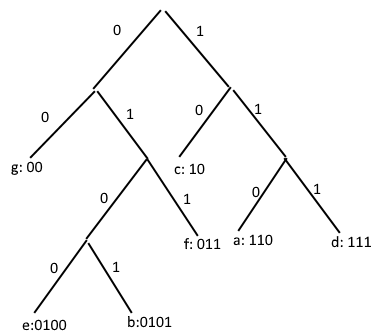
\includegraphics[width=\linewidth]{Huffman.png}
\caption{Иллюстрация к примеру.}
\label{fig:Huffman}
\end{figure}
\subsection{Самостоятельное изучение}
\subsubsection{Неравенство Крафта.}

Пусть задан набор длин $l_{1}, \ldots, l_{m}$, не все обязательно различные. Может ли такой набор оказаться набором длин некоторого префиксного кода? 

\textbf{Теорема.} Для того чтобы набор длин $l_{1}, \ldots, l_{m}$ мог быть набором длин кодовых последовательностей некоторого префиксного кода для алфавита из $m$ символов необходимо и достаточно, чтобы $\sum\limits_{i\in 1:m} 2^{-l_{i}} \leqslant 1$.

\textit{Доказательство.} Необходимость. Существует некоторый префиксный код для алфавита мощности $m$, кодовые последовательности которого имеют длины $l_{1}, \ldots, l_{m}$. Проверим выполнение неравенства Крафта. Обратимся к нашей интерпретации множества кодовых последовательностей как набор всех путей на двоичном дереве от корня к листу. Исходный, корневой, узел назовём нулевым уровнем, а дальше -- последовательно прибавляем номер уровня по мере удаления от нулевого. Каждому узлу $v$ на $t$-м уровне поставим в соответствие число $a(v) = 2^{-t}$ (тогда, например, корню соответствует $2^{-0} = 1$). 

Пусть мы нашли узел $v$ на уровне $t$, не являющийся листом, то есть на уровне $t+1$ есть хотя бы один узел, который получился после ветвения из данного -- назевём их $N(v)$ (это множество, состоящее из одного или двух элементов). Тогда, $a(v) \geqslant \sum\limits_{u \in N(v)} a(u)$ --- неравенство, если один узел, равенство, если два узла.

Просуммируем такие неравенства для каждого не листа: $$\sum\limits_{v \text{ не листья}} a(v) \geqslant \sum\limits_{u \text{ не корень}} a(u)$$.

$$2^{0} \geqslant \sum\limits_{u \text{ листья}} a(u).$$

Обратно, пусть выполнено неравенство. Пусть $l_{1}\leqslant \ldots \leqslant l_{m}$.

$n_{j}$ --- число листьев, которые должны оказаться на уровне $j$: $n_{j} = |\{i: l_{i} = j, i\in 1:m\}|$.

Известно, $$\sum\limits_{i\in 1:m} 2^{-l_{i}} \leqslant 1,$$ значит, $$\sum\limits_{j\in 1:l_{m}} 2^{-{j}} n_{j} \leqslant 1.$$

Тогда, для каждого $j\in 1:l_{m}$, $$n_{j} \leqslant 2^{j} - (2^{j-1}n_{1} +\ldots + 2 n_{j-1}).$$

Пусть $m \neq 1$ (случай одной вершины очевиден), рассмотрим $n_{1}$, выделим на первом уровне вершин $n_{1} \leqslant 2$, на втором уровне останется $2(2 - n_{1})$. Известно, что $n_{2} \leqslant 2^{2} - 2n_{1}$, значит, осталось не меньше, чем требуется для второго уровня.

Пусть на $(j-1)$-м уровне было свободно $$2^{j-1} - (2^{j-2} n_{1} +\ldots + 2 n_{j-2}),$$ известно, что $n_{j-1}$ не больше этой величины. Выделим $n_{j-1}$ узлов, останется $2^{j-1} - (2^{j-2} n_{1} +\ldots + 2 n_{j-2}) - n_{j-1}$, значит, на $j$-м уровне будет $2*(\ldots) =2^{j} - (2^{j-1}n_{1} +\ldots + 2 n_{j-1})$.

Таким образом, строится двоичное дерево с нужным количеством листьев на нужных уровнях, по которому восстановим префиксный код.
\subsection{15.02.19}
Примечание: здесь и далее (в том числе, в последующих лекциях) при введении условной вероятности мы подразумеваем, что нужные вероятности положительны, поэтому это условие будет опускаться.
\subsubsection{Конечная случайная схема и энтропия}
Пусть $A_1, A_2, \; ... \; , A_n$ - разбиение множества исходов S вероятностного пространства (S, Pr). \\
Конечной случайной схемой (КСС) называется схема $\alpha$, сопоставляющая каждому $A_i$ вероятность $Pr(A_i)$.\\
Энтропией КСС называется $H(\alpha) = -\sum\limits_{i = 1}^n Pr(A_i) * \log Pr(A_i)$.\\
Некоторые свойства энтропии:\\
\begin{itemize}
\item $H(\alpha) \geq 0$\\
\item Энтропия характеризует неопределенность, заключенную в КСС\\
\item Для любой КСС $\alpha$, у которой k исходов, $H(\alpha) \leq \log k$\\
Доказательство:\\
Обозначим $f(x) = -x * \log x$. На отрезке $[0, 1]$ $f(x)$ строго выпуклая, а значит, по неравенству Йенсена,\\
$\sum\limits_{i = 1}^n \lambda_i * f(x_i) \leq f(\sum\limits_{i = 1}^n \lambda_i * x_i)$, \\
Причем равенство достигается тогда и только тогда, когда $x_1 = \; ... \; = x_n$.\\
Тогда если взять $x_i = Pr(A_i)$ и $\lambda_i = \frac{1}{k}$ $\forall i \in 1..k$, получаем:\\
$\sum\limits_{i = 1}^k \frac{1}{k}(-Pr(A_i) * \log Pr(A_i)) \leq -\sum\limits_{i = 1}^k \frac{1}{k}Pr(A_i) * \log (\sum\limits_{i = 1}^k \frac{1}{k}Pr(A_i))$\\
$-\frac{1}{k} \sum\limits_{i = 1}^k Pr(A_i) * \log Pr(A_i) \leq -\frac{1}{k} \log\frac{1}{k}$\\
$-\sum\limits_{i = 1}^k Pr(A_i) * \log Pr(A_i) \leq \log k$\\
\item Из предыдущего пункта и условия равенства для неравенства Йенсена следует, что максимально возможную энтропию для КСС с k исходами, равную $\log k$, имеет схема с k равновероятными исходами.\\
\item $H(\alpha) = 0 \Leftrightarrow \exists!$ достоверный исход в $\alpha$. \\
Доказательство в обе стороны очевидно. Если в сумме, составляющей энтропию, есть хоть одно ненулевое слагаемое, то и энтропия ненулевая, а $x \log x = 0$ только при $x = 0$ и $x = 1$.
\end{itemize}
\subsubsection{Энтропия пересечения и условная энтропия}
Пусть есть две КСС - $\alpha$ с исходами $A_1, \; ... \; , A_k$ и $\beta$ с исходами $B_1, \; ... \; , B_l$. Их пересечением $\alpha \cap \beta$ называют схему, исходы которой - $A_i \cap B_j$ $\forall i \in 1..k, \forall j \in 1..l$.\\
Тогда $H(\alpha \cap \beta) = -\sum\limits_{i = 1}^k \sum\limits_{j = 1}^l Pr(A_i \cap B_j) * \log Pr(A_i \cap B_j)$\\
Воспользовавшись тем, что $Pr(A_i \cap B_j) = Pr(A_i) * Pr(B_j | A_i)$, получаем\\
$H(\alpha \cap \beta) = -\sum\limits_{i = 1}^k \sum\limits_{j = 1}^l Pr(A_i) * Pr(B_j | A_i) * (\log Pr(A_i) + \log Pr(B_j | A_i)) =$ \\ 
$ = -\sum\limits_{i = 1}^k \sum\limits_{j = 1}^l Pr(A_i) * Pr(B_j | A_i) * \log Pr(A_i) - \sum\limits_{i = 1}^k \sum\limits_{j = 1}^l Pr(A_i) * Pr(B_j | A_i) * \log Pr(B_j | A_i) = $\\
$ = -\sum\limits_{i = 1}^k Pr(A_i) * \log Pr(A_i) * \sum\limits_{j = 1}^l Pr(B_j | A_i) + \sum\limits_{i = 1}^k  Pr(A_i) * (-\sum\limits_{j = 1}^l Pr(B_j | A_i) * \log Pr(B_j | A_i)) = $\\
$ = -\sum\limits_{i = 1}^k Pr(A_i) * \log Pr(A_i) + \sum\limits_{i = 1}^k  Pr(A_i) * (-\sum\limits_{j = 1}^l Pr(B_j | A_i) * \log Pr(B_j | A_i)) = $\\
$ = H(\alpha) + \sum\limits_{i = 1}^k  Pr(A_i) * (-\sum\limits_{j = 1}^l Pr(B_j | A_i) * \log Pr(B_j | A_i))$.\\
$H(\beta | A_i) = -\sum\limits_{j = 1}^l Pr(B_j | A_i) * \log Pr(B_j | A_i)$ называют условной энтропией $\beta$ при условии $A_i$.\\
$H_{\alpha}(\beta) = \sum\limits_{i = 1}^k  Pr(A_i) * H(\beta | A_i)$ называют (средней) условной энтропией $\beta$ при условии $\alpha$.\\
Таким образом, в итоге формулу можно записать как \\
$H(\alpha \cap \beta) = H(\alpha) + H_{\alpha}(\beta)$.\\
Докажем, что  $0 \leq H_{\alpha}(\beta) \leq H(\beta)$:\\
Левая часть очевидна из тех же соображений, из которых следует неотрицательность энтропии.\\
чтобы доказать правую, напишем для зафиксированного j, функции $f(x) = -x * \log x$, $\lambda_i = Pr(A_i)$, $x_i = Pr(B_j | A_i)$ $\forall i \in 1..k$ неравенство Йенсена:\\
$\sum\limits_{i = 1}^k Pr(A_i) * (- Pr(B_j | A_i) * \log Pr(B_j | A_i)) \leq -(\sum\limits_{i = 1}^k Pr(A_i) * Pr(B_j | A_i)) * \log \sum\limits_{i = 1}^k Pr(A_i) * Pr(B_j | A_i)$\\
Преобразуем правую часть:\\
$-(\sum\limits_{i = 1}^k Pr(A_i) * Pr(B_j | A_i)) * \log \sum\limits_{i = 1}^k Pr(A_i) * Pr(B_j | A_i) = -(\sum\limits_{i = 1}^k Pr(B_j \cap A_i)) * \log \sum\limits_{i = 1}^k Pr(B_j \cap A_i) = -Pr(B_j) * \log Pr(B_j)$\\
После чего просуммируем обе части неравенства по j:\\
$\sum\limits_{j = 1}^l \sum\limits_{i = 1}^k Pr(A_i) * (- Pr(B_j | A_i) * \log Pr(B_j | A_i)) \leq \sum\limits_{j = 1}^l (-Pr(B_j) * \log Pr(B_j))$\\
$\sum\limits_{i = 1}^k Pr(A_i) * \sum\limits_{j = 1}^l (- Pr(B_j | A_i) * \log Pr(B_j | A_i)) \leq -\sum\limits_{j = 1}^l Pr(B_j) * \log Pr(B_j)$\\
$\sum\limits_{i = 1}^k Pr(A_i) * H(\beta | A_i) \leq H(\beta)$\\
$H_{\alpha}(\beta) \leq H(\beta)$.\\
Из условия равенства для неравенства Йенсена следует, что $H_{\alpha}(\beta) = H(\beta) \Leftrightarrow$ все $Pr(B_j | A_i)$ равны между собой.\\
По формуле полной вероятности,\\
$\forall j \in 1..l \; Pr(B_j) = \sum\limits_{i = 1}^k Pr(B_j | A_i) * Pr(A_i)$\\
Используя равенство всех $Pr(B_j | A_i)$ пишем:\\
$\forall j \in 1..l \; Pr(B_j) = Pr(B_j | A_1) * \sum\limits_{i = 1}^k Pr(A_i)$\\
$\forall j \in 1..l \; Pr(B_j) = Pr(B_j | A_1)$\\
То есть, $\forall i \in 1..k, \forall j \in 1..l \; Pr(B_j) = Pr(B_j | A_i)$
Вспомним теперь определение взаимно независимых событий:\\
A и B независимы $\Leftrightarrow Pr(A \cap B) = Pr(A) * Pr(B) \Leftrightarrow Pr(A) * Pr(B | A) = Pr(A) * Pr(B) \Leftrightarrow Pr(B | A) = Pr(B)$.\\
КСС $\alpha$ и $\beta$ называются независимыми, когда все исходы $\alpha$ независимы со всеми исходами $\beta$.\\
В таком случае, $H_{\alpha}(\beta)$ максимальна и равна $H(\beta)$.
\subsubsection{Количество информации}
Величина $I(\alpha, \beta) = H(\beta) - H_{\alpha}(\beta)$ называется количеством информации.\\
Запишем несколько свойств количества информации, которые доказываются простой проверкой:\\
\begin{itemize}
\item $I(\alpha, \beta) \geq 0$\\
\item $I(\alpha, \beta) = H(\beta) \Leftrightarrow H_{\alpha}(\beta) = 0$\\
\item $I(\alpha, \beta) = I(\beta, \alpha)$\\
\item $I(\alpha, \beta) = 0 \Leftrightarrow$ $\alpha$ и $\beta$ независимы.
\end{itemize}
Пример:\\
Загадано натуральное число $x \in 1..N$\\
$\beta$ - опыт, состоящий в нахождении x, $\beta_m$ - опыт, показывающий, делится ли x на m, $m \in 1..N$.\\
У $\beta$ N исходов, у $\beta_m$ два исхода.\\
$H_{\beta_m}(\beta) = Pr\{x \vdots m\} * H(\beta | "x \vdots m") + Pr\{x \not\vdots m\} * H(\beta | "x \not\vdots m")$\\
Если обозначить количество чисел от 1 до N, которые делятся на m, как $q = \lfloor \frac{N}{m} \rfloor$, то мы получим:\\
$Pr\{x \vdots m\} = \frac{q}{N}$\\
$Pr\{x \not\vdots m\} = \frac{N - q}{N}$\\
$H(\beta | "x \vdots m") = -\sum\limits_{i \vdots m, i \in 1..N} \frac{1}{q} * \log \frac{1}{q} = -\frac{q}{q} * \log \frac{1}{q} = \log q$\\
Аналогично $H(\beta | "x \not\vdots m") = \log (N - q)$\\
Таким образом, $H_{\beta_m}(\beta) = \frac{q}{N} * \log q + \frac{N - q}{N} * \log (N - q)$\\
$I(\beta_m, \beta) = \log N - \frac{q}{N} * \log q - \frac{N - q}{N} * \log (N - q) = $\\
$ = \frac{q}{N} * \log N - \frac{q}{N} * \log q + \frac{N - q}{N} * \log N - \frac{N - q}{N} * \log (N - q) = $\\
$ = -\frac{q}{N} * \log \frac{q}{N} - \frac{N - q}{N} * \log \frac{N - q}{N} \leq \log 2$\\
Равенство достигается при $q = N - q = \frac{N}{2}$, то есть если N четно и $m = 2$.

\subsection{22.02.19}
\subsubsection{Пример с данетками}
"Say 'what' again, I dare you, I dare you, I double-dare you, say 'what' one more goddamn time!"
Итак, загадано число от 1 до N, опыт $\beta$ - угадать число, опыт $\alpha$ - задать любой общий (да/нет) вопрос и получить ответ.\\
$H(\beta) = \log N$, поскольку с равной вероятностью было загадано каждое из N чисел.\\
$H(\alpha) \leq \log 2$, поскольку есть всего 2 варианта ответа.\\
Тогда $H(\alpha_1\alpha_2...\alpha_k) \leq \log 2^k = k \log 2$ (k вопросов, на каждый 2 варианта ответа).\\
А значит, чтобы угадать число, потребуется $k \geq \frac{\log N}{\log 2} = \log_2 N$ вопросов.\\
Есть ли какой-то алгоритм, который умеет-таки угадывать загаданное число за $O(\log N)$? Да. Называется бинпоиск (он же бинарный поиск, двоичный поиск).
\subsubsection{Пример с избыточным кодированием}
Итак, есть сообщение $u \in \{0, 1\}^k$, которое нужно передать. При этом мы можем передать сообщение $x(u) \in \{0, 1\}^n, n \geq k$, содержащее некоторую избыточную информацию. Зачем? Затем что канал связи "шумит" и может допускать ошибки. Конкретно, не более d ошибок на сообщение.\\
Итак, есть два сту... опыта: \\
$\beta$ заключается в нахождении всех d ошибок. Сколько у $\beta$ исходов? Для каждого количества ошибок j от 0 до d есть $(^n_j)$ вариантов их расположения, то есть всего исходов у $\beta$ $\sum\limits_{j = 0}^n (^n_j)$, откуда $H(\beta) = \log \sum\limits_{j = 0}^n (^n_j)$\\
$\alpha$ - это наше дополнительное сообщение размера $n - k$, соотвественно, таких сообщений всего $2^{n - k}$, а значит, $H(\alpha) = \log 2^{n - k} = (n - k) \log 2$.\\
Таким образом, чтобы суметь гарантированно найти все ошибки, нужно, чтобы $H(\alpha) \geq H(\beta)$. Отсюда\\
\begin{center}
$(n - k) \log 2 \geq \log \sum\limits_{j = 0}^n (^n_j)$\\
$n - k \geq \log_2 \sum\limits_{j = 0}^n (^n_j)$\\
$n \geq k + \log_2 \sum\limits_{j = 0}^n (^n_j)$\\
$k \leq n - \log_2 \sum\limits_{j = 0}^n (^n_j)$\\
\end{center}
Это значит, что если наш канал связи допускает не более d ошибок, чтобы передать сообщение размера k нам понадобится не менее $k + \log_2 \sum\limits_{j = 0}^n (^n_j)$ бит.\\
Или, что более естественно, поскольку количество ошибок обычно таки зависит от размера переданного сообщения (а еще потому что правая часть зависит от n, и выразить k значительно проще), если мы передаем n бит, и из них не более d могут быть ошибочными, в переданном сообщении можно закодировать сообщение длиной не более $n - \log_2 \sum\limits_{j = 0}^n (^n_j)$.
\subsubsection{Код Хэминга}
Частный случай предыдущей задачи при $d = 1$. Итак, как мы уже выяснили, $2^{n - k} \geq \sum\limits_{j = 0}^1 (^n_j) = 1 + n$. Сделав замену переменной $l = n - k$ (длина "избыточного" сообщения) получим $k \leq 2^l - l - 1$.
\begin{table}[H]
\caption{Максимальные значения k для фиксированных l}
\label{tabular:messageLengths}
\begin{center}
\begin{tabular}{|c|c|}
\hline
l & k\\
\hline
1 & 0\\
\hline
2 & 1\\
\hline
3 & 4\\
\hline
4 & 11\\
\hline
5 & 26\\
\hline
6 & 57\\
\hline
\end{tabular}
\end{center}
\end{table}
Как видно из таблицы, на совсем маленьких сообщениях все плохо, но чем больше сообщение, тем меньше (относительно) нужно лишней информации. Но как же так хитро передавать дополнительную информацию?\\
Итак, пусть $k = 12$ и мы хотим передать сообщение $u = 101101011100$. Нарисуем таблицу, j-м столбцом которой будет двоичная запись числа j (от младшего бита к старшему), размера 17 (по нашей таблице, для 12 бит сообщения 4 бит дополнительной информации уже мало, и надо брать 5, а $12 + 5 = 17$).\\
\begin{table}[H]
\caption{Двоичная матрица A}
\label{tabular:binaryCodes}
\begin{center}
\begin{tabular}{|c|c|c|c|c|c|c|c|c|c|c|c|c|c|c|c|c|}
\hline
l & 0 & 1 & 0 & l & 0 & 1 & 0 & l & 0 & 1 & 0 & l & 0 & 1 & 0 & 1\\
\hline
0 & 1 & 1 & 0 & 0 & 1 & 1 & 0 & 0 & 1 & 1 & 0 & 0 & 1 & 1 & 0 & 0\\
\hline
0 & 0 & 0 & 1 & 1 & 1 & 1 & 0 & 0 & 0 & 0 & 1 & 1 & 1 & 1 & 0 & 0\\
\hline
0 & 0 & 0 & 0 & 0 & 0 & 0 & 1 & 1 & 1 & 1 & 1 & 1 & 1 & 1 & 0 & 0\\
\hline
0 & 0 & 0 & 0 & 0 & 0 & 0 & 0 & 0 & 0 & 0 & 0 & 0 & 0 & 0 & 1 & 1\\
\hline
\end{tabular}
\end{center}
\end{table}
А теперь зарезервируем в нашем сообщении длины 17 места с номерами $2^i$ (1, 2, 4, 8, 16), а на остальные позиции запишем наше сообщение:\\
$x_0(u) = \_\_1\_011\_0101110\_0$\\
А теперь начинается магия: подберем на позицию $2^i$ такую цифру, чтобы произведение $x(u)$ и i-й строки матрицы было равно 0. Как же мы подберем, если в $x(u)$ еще куча неопределенных позиций? Да очень просто: на этих позициях в строчке с номером i стоят нули, потому что в двоичной записи числа $2^j$ единица стоит только на позиции j, а значит, при $i \not= j$ там стоит ноль, следовательно, что там будет стоять в итоговом виде $x(u)$ нам все равно. Отсюда же очевидно, что на позиции $2^i$ в i-й строчке будет всегда стоять единица.\\
Итак, подберем нужную цифру:\\
$? * 1 + \_ * 0 + 1 * 1 + \_ * 0 + 0 * 1 + 1 * 0 + 1 * 1 + \_ * 0 + 0 * 1 + 1 * 0 + 0 * 1 + 1 * 0 + 1 * 1 + 1 * 0 + 0 * 1 + \_ * 0 + 0 * 1 = ? + 1 + 1 + 1 = 1 + ? = 0$, откуда $? = 1$.\\
$x_1(u) = 1\_1\_011\_0101110\_0$\\
Аналогично заполняем остальные пропуски, получая $x(u) = 11110110010111000$.\\
Как же теперь понять, где была ошибка? Давайте испортим 10-ю позицию:\\
$y = 11110110000111000$\\
А теперь посчитаем $A \times y^T = \left( \begin{array}{c}
0 \\ 1 \\ 0 \\ 1 \\ 0 \end{array} \right)$\\
Получили двоичную запись (старший бит снизу) позиции, в которой произошла ошибка: $2^1 + 2^3 = 10$. Как?\\
При умножении на i-ю строку матрицы j-я позиция сообщения влияла только если $A[i][j] = 1$, то есть если на i-м месте в двоичной записи числа j стояла единица. Поэтому результат произведения строки матрицы на столбец сообщения изменился (став единицей) только для тех строк, где на 10-й позиции стояла единица (а это строки с номерами, равными позициям, где в двоичной записи числа 10 стоят единицы), а для остальных строк остался нулем.

\subsection{28.02.19}
\subsubsection{Случайные процессы, цепи}
В целом, процесс - это изменение некоторой системы с течением времени (плавление металла, движение тела, брошенного под углом к горизонту, сон студента на паре). Но рассматривать непрерывные процессы, в которых у системы континуум состояний нам как-то не с руки, поэтому вводится некоторая математическая модель:\\
Пусть есть дискретное время $T \subseteq \mathbb{N}$, пространство состояний системы $M$. Тогда случайным процессом (с дискретным временем, другие мы рассматривать, надеюсь, не будем) называется последовательность ${\xi_n, n \in T}$, где $\forall n \in T \; Im(\xi_n) \subseteq M, \sum\limits_{s \in M} Pr\{\xi_n = s\} = 1$. Вообще говоря, $M$ может не быть дискретным, и тогда $\xi_n$ будут непрерывными случайными величинами, но у нас такого не будет, поэтому $M$ всегда не более чем счетно, и $\xi_n$ тогда будут ДСВ. Случайный процесс с дискретным временем называют также случайной цепью.\\
Траекторией длины n случайного процесса называют последовательность $r_0, \; ... \; , r_n$ такую, что $\xi_i = r_i \; \forall i \in 0:n$ - первое $n + 1$ (либо "длина" тут относится к количеству смен состояний, либо я просто криво записал) состояние, через которое прошла система.\\
Пример: случайные блуждания по точкам с целой координатой числовой прямой. Если в данный момент мы стоим в точке с координатой $x$, то с вероятностью $p$ мы переходим в точку $x + 1$, и c вероятностью $1 - p$ - в $x - 1$.\\
В этом процессе $Pr\{\xi_n = x | \xi_0 = x_0, \; ... \; \xi_{n - 1} = x_{n - 1}\} =  p$, если $x_{n - 1} + 1 = x$, $1 - p$, если $x_{n - 1} - 1 = x$ и 0 иначе.
\subsubsection{Марковские цепи}
Заметим, что в предыдущем примере распределение $\xi_n$ зависит только от значения $\xi_{n - 1}$, но не от предыдущих состояний системы и n. Иными словами, $Pr\{\xi_n = x | \xi_0 = x_0, \; ... \; , \xi_{n - 1} = x_{n - 1}\} = Pr\{\xi_n = x | \xi_{n - 1} = x_{n - 1}\}$.\\
Такие процессы, пространство состояний которых конечно, и в которых $\forall x_0, x_1, \; ... \; , x_{n - 1}, i, j \in M \; Pr\{\xi_{n + 1} = j | \xi_0 = x_0, \; ... \; , \xi_n = i\} = P_{i, j}$, где P - матрица переходных вероятностей - Стохастическая (по строкам) матрица (то есть, такая, что сумма всех значений на любой строке равна 1, и все эти значения неотрицательны) размера $|M| \times |M|$, называются Марковскими процессами или цепями (вообще говоря, Марковский процесс не обязательно имеет дискретное время, но поскольку процессы с непрерывным временем мы не рассматриваем, то для нас это синонимы).\\
Пример: напишем матрицу переходных вероятностей для процесса бросания монетки, пока не выпадет 5 орлов (считаем, что если 5 орлов уже выпало, то мы с вероятностью 1 остаемся в этом состоянии).\\
\begin{table}[H]
\caption{Матрица переходных состояний.}
\label{tabular:TransitionStatesMatrix}
\begin{center}
\begin{tabular}{|c|c|c|c|c|c|c|}
\hline
$\cdot$ & 0 & 1 & 2 & 3 & 4 & 5\\
\hline
0 & $\frac{1}{2}$ & $\frac{1}{2}$ & 0 & 0 & 0 & 0\\
\hline
1 & 0 & $\frac{1}{2}$ & $\frac{1}{2}$ & 0 & 0 & 0\\
\hline
2 & 0 & 0 & $\frac{1}{2}$ & $\frac{1}{2}$ & 0 & 0\\
\hline
3 & 0 & 0 & 0 & $\frac{1}{2}$ & $\frac{1}{2}$ & 0\\
\hline
4 & 0 & 0 & 0 & 0 & $\frac{1}{2}$ & $\frac{1}{2}$\\
\hline
5 & 0 & 0 & 0 & 0 & 0 & 1\\
\hline
\end{tabular}
\end{center}
\end{table}
\subsection{01.03.19}
\subsubsection{Свойства Марковских цепей}
\begin{itemize}
\item $Pr\{\xi_{n + 1} = j | \xi_0 = i_0, \; ... \; , \xi_n = i\} = Pr\{\xi_{n + 1} = j | \xi_n = i\}$\\
Доказательство:\\
$Pr\{\xi_{n + 1} = j | \xi_n = i\} = \frac{Pr\{\xi_{n + 1} = j, \xi_n = i\}}{Pr\{\xi_n = i\}} = \sum\limits_{(i_0, ..., i_{n-1}) \in M^n} \frac{Pr\{\xi_{n+1} = j, \xi_n = i, \xi_0 = i_0, \; ... \; , \xi_{n - 1} = i_{n - 1}\}}{Pr\{\xi_n = i\}} = \sum\limits_{(i_0, ..., i_{n-1}) \in M^n} \frac{Pr\{\xi_{n + 1} = j, \xi_n = i, \xi_0 = i_0, \; ... \; , \xi_{n - 1} = i_{n - 1}\}}{Pr\{\xi_n = i\}} = \sum\limits_{(i_0, ..., i_{n-1}) \in M^n} \frac{P_{ij}Pr\{\xi_n = i, \xi_0 = i_0, \; ... \; , \xi_{n - 1} = i_{n - 1}\}}{Pr\{\xi_n = i\}} = \frac{P_{ij}}{Pr\{\xi_n = i\}} * \sum\limits_{(i_0, ..., i_{n-1}) \in M^n}Pr\{\xi_n = i, \xi_0 = i_0, \; ... \; , \xi_{n - 1} = i_{n - 1}\} = \frac{P_{ij}}{Pr\{\xi_n = i\}} * Pr\{\xi_n = i\} = P_{ij}$\\
\item $Pr\{\xi_{n + 1} = j | \xi_k = i_k, \xi_n = i\} = Pr\{\xi_{n + 1} = j | \xi_n = i\}$\\
(Никакие состояния, кроме предыдущего, не влияют на вероятность перехода).\\
\item $Pr\{\xi_{n + m} = j | \xi_0 = i_0, \; ... \; , \xi_n = i\} = Pr\{\xi_{n + m} = j | \xi_n = i\}$\\
Доказательство:\\
Для $m = 1$ утверждение уже доказано.\\
Пусть утверждение верно для $m = k$, докажем его для $m = k + 1$:\\
$Pr\{\xi_{n + k + 1} = j | \xi_0 = i_0, \; ... \; , \xi_n = i\} = \frac{Pr\{\xi_{n + k + 1} = j, \xi_0 = i_0, \; ... \; , \xi_n = i\}}{Pr\{\xi_0 = i_0, \; ... \; , \xi_n = i\}} = \sum\limits_{s \in M} \frac{Pr\{\xi_{n + k + 1} = j, \xi_{n + k} = s, \xi_0 = i_0, \; ... \; , \xi_n = i\}}{Pr\{\xi_0 = i_0, \; ... \; , \xi_n = i\}} = \sum\limits_{s \in M} \frac{P_{sj}Pr\{\xi_{n + k} = s, \xi_0 = i_0, \; ... \; , \xi_n = i\}}{Pr\{\xi_0 = i_0, \; ... \; , \xi_n = i\}} = \sum\limits_{s \in M} P_{sj}Pr\{\xi_{n + k} = s | \xi_0 = i_0, \; ... \; , \xi_n = i\} = \sum\limits_{s \in M} Pr\{\xi_{n + k + 1} = j | \xi_{n + k} = s\}Pr\{\xi_{n + k} = s | \xi_n = i\} = \sum\limits_{s \in M} \frac{Pr\{\xi_{n + k + 1} = j | \xi_{n + k} = s, \xi_{n} = i\}Pr\{\xi_{n + k} = s, \xi_n = i\}}{Pr\{\xi_n = i} = \sum\limits_{s \in M} \frac{Pr\{\xi_{n + k + 1} = j, \xi_{n + k} = s, \xi_n = i\}}{Pr\{\xi_n = i} = \sum\limits_{s \in M} \frac{Pr\{\xi_{n + k} = s | \xi_{n + k + 1} = j, \xi_n = i\}Pr\{\xi_{n + k + 1} = j, \xi_n = i\}}{Pr\{\xi_n = i} = \frac{Pr\{\xi_{n + k + 1} = j, \xi_n = i\}}{Pr\{\xi_n = i} \sum\limits_{s \in M} Pr\{\xi_{n + k} = s | \xi_{n + k + 1} = j, \xi_n = i\} = Pr\{\xi_{n + k + 1} = j | \xi_n = i\} * 1 = Pr\{\xi_{n + k + 1} = j | \xi_n = i\}$\\
\item Однородность: $Pr\{\xi_{n + 1} = j | \xi_n = i\} = P_{ij} = Pr\{\xi_1 = j | \xi_0 = i\}$\\
\item $Pr\{\xi_{n + m} = j | \xi_n = i\} = Pr\{\xi_m = j | \xi_0 = i\}$
\item $\forall n > 0 \; Pr\{\xi_n = i\} = \sum\limits_{s \in M} Pr\{\xi_n = i | \xi_0 = s\}$\\
\end{itemize}
\subsubsection{Матрица перехода на n шагов}
$P = P(1)$ - матрица перехода на 1 шаг.\\
$P(n): \; P(n)_{ij} = Pr\{\xi_n = j | \xi_0 = i\}$ - матрица перехода на n шагов.\\
Лемма: произведение двух стохастических (по строкам) матриц - также стохастическая матрица. Доказать самостоятельно (на экзамене не будет).\\
Свойство: $P(m + n) = P(m)P(n)$ (откуда получаем, что $P(n) = P(1)^n)$.\\
Доказательство: \\
$P(m + n)_{ij} = Pr\{\xi_{m + n} = j | \xi_0 = i\} = \sum\limits_{s \in M}Pr\{\xi_{m + n} = j | \xi_m = s\}Pr\{\xi_{m} = s | \xi_0 = i\} = \sum\limits_{s \in M} P(m)_{is}P(n)_{sj}$\\
\subsubsection{Пример со скрещиванием гибридов.}
Пусть G и g - две формы одного гена. Любой организм содержит два таких гена - GG, Gg или gg. Каждый потомок получает по одному гену от каждого из родителей равновероятно (то есть, у GG и Gg с вероятностью $\frac{1}{2}$ родится потомок Gg и с вероятностью $\frac{1}{2}$ - GG). Напишем матрицу переходных состояний P при скрещивании с гибридом (Gg):\\
\begin{table}[H]
\caption{Матрица переходных состояний.}
\label{tabular:TransitionStatesMatrix}
\begin{center}
\begin{tabular}{|c|c|c|c|}
\hline
$\cdot$ & gg & Gg & GG\\
\hline
gg & $\frac{1}{2}$ & $\frac{1}{2}$ & 0\\
\hline
Gg & $\frac{1}{4}$ & $\frac{1}{2}$ & $\frac{1}{4}$\\
\hline
GG & 0 & $\frac{1}{2}$ & $\frac{1}{2}$\\
\hline
\end{tabular}
\end{center}
\end{table}
Пусть исходный организм мог с равной вероятностью иметь любой набор генов. Тогда распределение исходного состояния $\mu = (\frac{1}{3}, \frac{1}{3}, \frac{1}{3})$.\\
$\mu * P = a = (\frac{1}{4}, \frac{1}{2}, \frac{1}{4})$\\
$\mu * P^2 = a$\\
Это явление называется стабилизацией Марковского процесса, а распределение a - стационарным распределением.
\subsubsection{Стабилизация и стационарное распределение}
Более формально, если существует $\lim\limits_{t \to +\infty} \mu * P^t = \pi$, $\pi$ называют стационарным распределением Марковской цепи.\\
Заметим, что $\pi = \lim\limits_{t \to +\infty} \mu * P^{t - 1} * P = \pi * P$.\\
\subsubsection{Эргодические Марковские цепи}
Если матрица P переходных состояний некой Марковской цепи такова, что $\exists n: \; \forall j \in M \; \exists i \in M: \; P^n_{ij} > 0$, то эта цепь называется эргодической, а P называется эргодической матрицей.\\
Теорема (без доказательства): Если Марковская цепь эргодическая, то у нее существует единственное стационарное распределение.
\subsection{15.03.19}
Замечание: для понимания этой лекции необходимо знание некоторых определений из следующего раздела.
\subsubsection{Классификация состояний Марковской цепи}
Пусть есть Марковская цепь с множеством состояний S и матрицей переходных вероятностей P, $i, j \in S$.
Говорят, что состояние j достижимо из состояния i ($i \rightarrow j$), если $\exists n \geq 0: \; P^n_{ij} > 0$.\\
Достижимость: \\
\begin{itemize}
\item рефлексивна: $P^0_{ii} = E_{ii} = 1 > 0$\\
\item транзитивна: $i \rightarrow j, j \rightarrow k \Rightarrow \exists m, n \in N_0: \; P^m_{ij} > 0, P^n_{jk} > 0 \Rightarrow P^{n + m}_{ik} = \sum\limits_{l \in S} P^m_{il}P^n_{lk} \geq P^m_{ij}P^n_{jk} > 0$.\\
\end{itemize}
Если $i \rightarrow j$ и $j \rightarrow i$, говорят, что состояния i и j сообщаются ($i \leftrightarrow j$).\\
Отношение сообщения, очевидно, симметрично, а значит, является отношением эквивалентности.\\
Значит, S разбивается на непересекающиеся классы сообщающихся вершин - классы эквивалентности по отношению сообщения.
Очевидно, что при представлении Марковской цепи в виде графа (вершины - состояния, веса ребер - переходные вероятности) классы сообщающихся вершин будут компонентами сильной связности.
Граф, построенный на компонентах сильной связности, ациклический, а значит, существует частичный порядок компонент сильной связности, задаваемый отношением достижимости (если компонента A достижима из компоненты B, то B "меньше" A).\\
Максимальные элементы в таком частичном порядке называются эргодическими классами, а состояния Марковской цепи, попавшие в какой-либо эргодический класс, называются возвратными.\\
Теорема (без доказательства):\\
Пусть $\xi_0 = i \in S$, причем i лежит в каком-то эргодическом классе.\\
$\tau_i$ - первый момент дискретного времени, когда марковский процесс вернется в состояние i, начавшись из i ($\tau_i > 0$). Утверждается, что $Pr\{\tau_i < \infty\} = 1$.\\
Все состояния, не являющиеся возвратными, называют несущественными.\\
Если граф Марковской цепи состоит из единственного эргодического класса, Марковская цепь неприводима (пример про скрещивание с гибридом).\\
Если некоторый эргодический класс состоит из одной вершины, это состояние называют поглощающим (пример ниже).
\subsubsection{Пример со случайным блужданием и поглощающими состояниями}
Пусть множество состояний - натуральные числа от 1 до N. Вероятность перейти в соседнее справа число - p, в соседнее слева - $1 - p$. Однако, состояния 1 и N являются поглощающими, то есть, при попадании в них мы с вероятностью 1 останемся в них же. Или, более формально,\\
$S = 0:N$, $P_{00} = P_{NN} = 1$, $P_{(i - 1)i} = p$, $P_{(i + 1)i} = 1 - p$.
Можно самостоятельно нарисовать граф для этого примера, а также для примера с бросанием монетки до 5 орлов (состояние 5 орлов считаем поглощающим) и примера про скрещивание с гибридом.
\subsubsection{Периодичность класса сообщающихся состояний}
Для состояния $i \in S$ рассмотрим множество $\rho_i = \{n \in N: \; P^n_{ii} > 0\}$.\\
$d(i) = \gcd(\rho_i)$ называют периодом состояния i.\\
В предыдущем примере $d(0) = d(N) = 1, \forall i \in 1:(N - 1) \; d(i) = 2$.\\
Если $d(i) = 1$, состояние i называют непериодическим.\\
Лемма:\\
Периоды сообщающихся состояний равны (а значит, период - свойство класса сообщающихся состояний).\\
Доказательство:\\
Пусть $i, j \in S, i \leftrightarrow j \Rightarrow \exists m, n \in N: \; P^m_{ij} > 0, P^n_{ji} > 0$.\\
$\forall d$ - делитель $\rho_i$, $\forall k \in \rho_j \; P^k_{jj} > 0$.\\
$P^{m + k + n}_{ii} \geq P^m_{ij}P^k_{jj}P^n_{ji} > 0 \Rightarrow (m + k + n) \in \rho_i \Rightarrow (m + k + n) \vdots d$.\\
При этом, $P^{m + n}_{ii} \geq P^m_{ij}P^n_{ji} > 0 \Rightarrow (m + n) \in \rho_i \Rightarrow (m + n) \vdots d$.\\
Если $(m + n) \vdots d$ и $(m + n + k) \vdots d$, значит, $k \vdots d$, то есть любой элемент $\rho_j$ делится на любой делитель $\rho_i$, а значит, $d(j) = \gcd(\rho_j) \geq \gcd(\rho_i) = d(i)$.\\
Аналогично, $d(i) \geq d(j)$, а значит, $d(i) = d(j)$, что и требовалось доказать.\\
Утверждение (без доказательства):\\
Если $d(i) < \infty$, то $\exists N: \; \forall n \geq N \; P^{n * d(i)}_{ii} > 0$.\\
Частный случай: $d(i) = 1 \Leftrightarrow \exists N: \; \forall n > N \; P^n_{ii} > 0$.

\section{Графы}
\subsection{15.03.19}
\subsubsection{Орграф}
Ориентированным графом или орграфом называют $G = (V, E)$, где $V \not= \varnothing$ - (конечное) множество вершин, а $E \subseteq V \times V$ - множество ребер.\\
Ребра часто записываются по их концам: $(v_1, v_2)$ или просто $v_1v_2$.\\
Множество вершин графа $G$ обозначают $V(G)$.\\
Множество ребер графа $G$ обозначают $E(G)$.\\
Примечание: \\
Хотя $V = \varnothing$ технически незаконно, иногда оно встречается в доказательствах.\\
Пустым графом называют граф, множество ребер которого пусто.\\
\subsubsection{Подграф}
Пусть $G = (V, E)$. $G' = (V', E')$ называют подграфом $G$ ($G'\leq G$), если $V' \subseteq V, E' \subseteq (V' \times V') \cap E$.\\
Если $E' = (V' \times V') \cap E$, подграф называют порожденным. Порожденный подграф обозначают $G[V']$.\\
\subsubsection{Пути и циклы}
Пусть $G = (V, E)$.\\
Путем называется последовательность вершин $v_0v_1...v_n: \; \forall i \in 0:n \; v_i \in V, \forall i \in 1:n \; (v_{i - 1}, v_i) \in E$.\\
Простым называется путь, в котором все вершины различны. Поскольку непростые пути в задачах встречаются редко, здесь и далее слово "путь" обозначает простой путь, если не указано обратного.\\
Циклом называется последовательность вершин $v_0v_1...v_n: \; \forall i \in 0:n \; v_i \in V, (v_i, v_{i + 1}) \in E, v_0 = v_n$.\\
Простым называется цикл, все вершины которого, кроме последней, различны. Так же как и с путями, слово "цикл" обозначает простой цикл, если не указано обратного.\\
Ациклическим графом называется орграф без циклов.
\subsubsection{Связность}
$Вершины u, v \in V(G)$ связаны между собой в графе G, если существует путь из $u$ в $v$.\\
Cильно связным называется такой граф $G$, что $\forall u, v \in V(G)$ $u$ связана с $v$ и $v$ связана с $u$.\\
Наибольший по включению сильно связный порожденный подграф называется компонентой сильной связности.\\
Отношение сильной связности, очевидно, рефлексивно (путь из одной вершины легален), транзитивно (простая проверка) и симметрично (по построению), а значит, компоненты сильной связности - это классы эквивалентности, то есть, они либо не пересекаются, либо совпадают.\\
Построим новый граф, в котором вершины соответствуют компонентам сильной связности старого и в новом графе из вершины $A$ в вершину $B$ существует ребро, если в исходном графе в компоненте, соответствующей $A$, была вершина $a$, а в компоненте, соответствующей $B$ - вершина $b$ такие, что $ab$ - ребро исходного графа.\\
Заметим, что построенный граф ациклический. (простая проверка от противного).\\
В ациклическом орграфе все компоненты сильной связности состоят из одной вершины.\\
Отношение связности в ациклическом графе, следовательно, рефлексивно, транзитивно и антисимметрично.\\
Значит, оно является отношением частичного порядка, а значит, существует топологическая сортировка.

\subsection{22.03.19}
\subsubsection{Неорграфы}
$2_V = \{\{u, v\}: \; u, v \in V\}$.\\
Неориентированным графом (неорграфом) называется пара $G = (V, E)$, где $V \not= \varnothing$ - (конечное) множество вершин, а $E \subseteq 2_V$ - множество ребер.\\
Замечание: штрихи, волны, точки и прочая ересь в обозначениях "наследуются"\, то есть мы по умолчанию считаем, что $V'$, например - множество вершин графа $G'$, а множество ребер этого графа - $E'$.\\
Ребра часто записываются по их концам: $(v_1, v_2)$ или просто $v_1v_2$.
Возможна запись $V(G)$ и $E(G)$.
Примечание: \\
хотя $V = \varnothing$ технически незаконно, иногда оно встречается в доказательствах.\\
Пустым графом называют граф, множество ребер которого пусто.\\
Пути, простые пути, циклы, простые циклы, подграфы и порожденные подграфы определяются так же, как для орграфов, с поправкой на замену $V \times V$ на $2_V$.\\
Примечание: цикл $v_1v_2v_1$ в этом определении считается законным, хотя по-моему это контринтуитивно.\\
$u, v \in V$ называются смежными, если $uv \in E$.
\subsubsection{Связность}
Неорграф называется связным, если между любыми двумя его вершинами существует путь.\\
Компонентой связности называется максимальный по включению связный порожденный подграф.\\
По тем же соображениям, что и с компонентами сильной связности, компоненты связности либо совпадают, либо не пересекаются.\\
Утверждение: если $G = (V, E)$ - связный граф, то существует нумерация вершин $v_1, v_2, \; ... \; , v_n$ такая, что $\forall i \in 1:n \; G_i = G[\{v_1, \; ... \; , v_i\}]$ - связный.\\
Доказательство:\\
база индукции - граф из одной вершины связен по определению.\\
шаг индукции - пусть $G_1, \; ... \; , G_i$ построены и связны.\\
Пусть $v \in V \setminus \{v_1, \; ... \; , v_i\}$ (если разность пуста, то $i = n$ и утверждение уже доказано).\\
В силу связности G существует путь $x_0x_1...x_m$, где $x_0 = v, x_m = v_1$.\\
$s = \max\{j \in 0:(m - 1) : \; x_j \not\in \{v_1,\;...\;, v_i\}\}$. Тогда положим $v_{i + 1} = x_s$. $G_{i + 1}$, очевидно, связный.\\
\subsubsection{Деревья}
Связный неорграф без циклов называется деревом.\\
Для следующего утверждения нам нужно научиться удалять и добавлять ребра.\\
Пусть $G = (V, E), \; u, v \in V$. \\
$G - uv = (V, E \setminus \{uv\})$\\
$G + uv = (V, E \cup \{uv\})$\\\\\\\\
Утверждение: следующие условия эквивалентны:\\
\begin{enumerate}
\item T - дерево.\\
\item Любые две вершины T соединяются единственным путем.\\
\item T - минимальный связный граф (в том смысле, что удаление любого ребра нарушит связность).\\
\item T - максимальный граф без циклов (в том смысле, что добавление любого ребра создаст цикл).\\
\end{enumerate}
Доказательство:\\
$1 \Rightarrow 2$) Любые две вершины соединяются хотя бы одним путем, так как дерево связно. Путей не может быть больше одного, так как если есть два различных пути, то из их объединения можно вычленить цикл (это очень нестрого и нужно бы формализовать).\\
$2 \Rightarrow 3$) Если удалить ребро $uv$, то поскольку это был единственный путь между u и v, эти две вершины больше не будут связными.\\
$3 \Rightarrow 4$) В минимальном связном графе нет циклов, так как иначе удаление любого ребра из цикла не нарушает связности. Добавление ребра $uv$ создает цикл, так как между u и v уже был путь.\\
$4 \Rightarrow 1$) Максимальный граф без циклов связен (и, как следствие, является деревом) так как если бы какие-то две вершины u и v нельзя было соединить путем, добавление ребра uv не создавало бы циклов.\\
Произвольный граф без циклов называют лесом (потому что каждая его компонента связности - дерево).\\
\subsubsection{Остовные деревья}
$H \leq G$ называют остовом G, если $V(H) = V(G)$.\\
Утверждение:\\
У каждого графа существует остовный лес (а у связного графа - остовное дерево), не увеличивающее количество компонент связности.\\
Доказательство:\\
Докажем только утверждение про связный граф, так как для несвязного графа можно по отдельности рассмотреть компоненты связности.\\
Для связного графа вспомним чудесную нумерацию из пункта про связность. Будем для каждого $i > 1$ брать ровно одно ребро, связывающее $v_i$ с $G_{i - 1}$. В графе не будет циклов, так как из каждой вершины только одно ребро ведет в вершину с меньшим номером, а если предположить, что цикл таки существует, у вершины с наибольшим номером в цикле должно быть два ребра в вершины с меньшими номерами. Ну и связность построенного графа можно проверить по индукции.\\
Утверждение:\\
(надеюсь, я правильно его понял)\\
Пусть T - дерево, тогда существует такая нумерация вершин $V(T) = \{v_1, \; ... \; , v_n\}$, что $\forall i \in 1:n \; \exists! j \in 1:(i - 1)$ такое, что $v_iv_j \in E(T_i)$, где $T_i = T[\{v_1, \; ... \; , v_i\}]$.\\
Доказательство:\\
Так как T связный, существует такая нумерация, что все $T_i$ связные.\\
В частности, поскольку $T_i$ связный, существует хотя бы одна вершина в $\{v_1, \; ... \; , v_{i - 1}\}$ смежная с $v_i$\\
Если есть две вершины в $\{v_1, \; ... \; , v_{i - 1}\}$ смежные с $v_i$, то поскольку $T_{i - 1}$ связный, это означает наличие цикла в T, чего быть не может.\\
Значит, такая вершина ровно одна.\\
Утверждение: связный граф на n вершинах дерево $\Leftrightarrow$ в нем ровно $n - 1$ ребро.\\
$\Rightarrow$) очевидно следует из нумерации.\\
$\Leftarrow$) Исходный граф $G: |V(G)| = n, |E(G)| = n - 1$. Из следствия, так как граф связный, он имеем остовное дерево $T: |V(T)| = n, |E(T)| = n - 1 \Rightarrow G = T \Rightarrow G$ - дерево\\
\subsubsection{Минимальное остовное дерево}
Введем функцию $w: \; E(G) \rightarrow R_+$ - веса ребер.\\
Вес графа $w_G = \sum\limits_{e \in E}w(e)$\\
Минимальным остовным деревом называется остовное дерево с минимальным весом.\\
Основная лемма об остовных деревьях:\\
Пусть $\mathcal{T}$ - множество всех минимальных остовных деревьев связного графа G.\\
$T \in \mathcal{T}, X \subseteq E(T)$. Пусть $\varnothing \not= S \subseteq V(G)$, $Q = \{uv: \; u \in S, v \in V(G) \setminus S\}$, причем $X \cap Q = \varnothing$.\\
Выберем $e \in Q: \; w(e) = \min\limits_{q \in Q}w(q)$. Тогда $\exists T' \in \mathcal{T}: \; X \cup \{e\} \in E(T')$\\
Доказательство:\\
Если $e \in E(T)$, $T' = T$. Иначе $T + e$ содержит цикл (поскольку дерево - максимальный граф без циклов).\\
Тогда $\exists e' \in E(T): \; e' \in Q$. $e' \not\in X$, так как $X \cap Q = \varnothing$.\\
$T' = T + e - e'$ - остовное дерево (вершины мы не удаляли, связность не нарушалась, так как удалили ребро из цикла.\\
Так как $w(e) = \min\limits_{q \in Q}w(q)$, то $w(e) \leq w(e')$ и $w(T') = w(T) + w(e) - w(e') \leq w(T)$, а значит, поскольку $T$ - минимальное остовное дерево, $T'$ - также минимальное остовное дерево.

\subsection{29.03.19}
\subsubsection{Алгоритм Прима-Ярника.}
Прекрасно описан на \href{http://www.e-maxx-ru.1gb.ru/algo/mst_prim}{E-maxx}.
\subsubsection{Алгоритм Краскала.}
\href{http://www.e-maxx-ru.1gb.ru/algo/mst_kruskal}{Там же}.
\subsubsection{Поток.}
Пусть у нас есть граф G.\\
$\forall e \in E(G) \; e = xy$ определим $\overrightarrow{e} = (e, x, y), \; \overleftarrow{e} = (e, y, x)$.\\
$\overrightarrow{E} = \{(e, x, y): \; e = xy; x, y \in V(G); e \in E(G)\}$ - заметим, что сюда входят ребра в обе стороны.\\
$|\overrightarrow{E}| = 2|E(G)|$.\\
Для двух подмножеств множества вершин $X, Y \subseteq V(G)$ определим $\overrightarrow{E}(X, Y) = \{(e, x, y): \; x \in X; y \in Y; (e, x, y) \in \overrightarrow{E}\}$.\\
Для любой функции $f: \; \overrightarrow{E} \rightarrow \mathbb{R}$ определим $\forall X, Y \subseteq V(G) \; f(X, Y) = \sum\limits_{\overrightarrow{e} \in \overrightarrow{E}(X, Y)}f(\overrightarrow{e})$.\\
Итак, пусть имеется произвольный неорграф G. Выделим в нем две вершины $s, t \in V(G); s \not= t$, s назовем истоком, а t - стоком.\\
Введем также на этом графе функцию $c: \; \overrightarrow{E} \rightarrow \mathbb{N}_0$ - пропускные способности ребер.\\
Тогда $(G, s, t, c)$ называют сетью.\\
Функция $f: \; \overrightarrow{E} \rightarrow \mathbb{R}$ является потоком в сети $(G, s, t, c)$, если:\\
\begin{itemize}
\item $\forall e \in E(G) \; f(\overrightarrow{e}) = f(\overleftarrow{e})$ \\
\item $\forall v \in V(G), v \not= s, v \not= t \; f(\{v\}, V(G)) = 0$ (если немного порисовать, станет понятно, что это условие означает, что для любой вершины сумма входящих потоков равна сумме исходящих, такое себе правило Киргхофа)\\
\item $\forall \overrightarrow{e} \in \overrightarrow{E} \; f(\overrightarrow{e}) \leq f(\overrightarrow{e})$
\end{itemize}
\subsubsection{Разрез.}
Разрезом в сети $(G, s, t, c)$ называют пару $(S, V(G) \setminus S)$, где $S \subset V(G), s \in S, t \not\in S$.\\
Утверждение: $\forall S \subset V(G) \; f(S, \overline{S}) = f(\{s\}, V(G))$.\\
Доказательство: $f(S, \overline{S}) = f(S, V) - f(S, S) = f(\{s\}, V) + f(S \setminus \{s\}, V) - f(S, S)$.\\
Второе слагаемое обнуляется по второму свойству из определения потока, третье - по третьему (ведь для любого ребра, поток по которому мы будем прибавлять, мы будем прибавлять и поток по обратному ребру).\\
$f(\{s\}, V) = f(S, \overline{S}) = |f|$ называют величиной потока в сети.\\
$c(S, \overline{S})$ - пропускная способность разреза.\\
Лемма: $|f| \leq c(S, \overline{S}) \; \forall f, (S, \overline{S})$.\\
Доказательство: $|f| = f(S, \overline{S}) = \sum\limits_{\overrightarrow{e} \in\overrightarrow{E}(S, \overline{S})}f(\overrightarrow{e} \leq \sum\limits_{\overrightarrow{e} \in\overrightarrow{E}(S, \overline{S})}c(\overrightarrow{e} = c(S, \overline{S})$.
\subsubsection{Теорема Форда-Фалкерсона.}
Теорема: $\max |f| = \min c(S, \overline{S})$.
Доказательство: "$\leq$" уже доказано в лемме.\\
$f_0$ - нулевой поток (поток на всех ребрах равен нулю).\\
$f_n$ - целочисленный поток.\\
$S_n = \{v \in V(G): \; s = v_0,v_1,...,v_n = v$ - простой путь, причем $(e_i, v_i, v_{i + 1}) = \overrightarrow{e_i} \in \overrightarrow{E}, c(\overrightarrow{e}) - f_n(\overrightarrow{e}) > 0 \}$ - множество вершин, достижимых из s по ребрам с ненулевой остаточной пропускной способностью.\\
Пусть $t \in S_n$.\\
$w = \{s = v_0, v_1, ... , v_l = t\}$ - путь по ребрам с ненулевой остаточной пропускной способностью.\\
$\epsilon = \min\limits_{i \in 0..(n - 1)} (c(\overrightarrow{e_i}) - f_n(\overrightarrow{e_i}))$, где $\overrightarrow{e_i} = (e_i, v_i, v_{i + 1})$.\\
Определим $f_{n + 1}$:\\
\begin{itemize}
\item $f_{n + 1}(\overrightarrow{e}) = f_{n}(\overrightarrow{e}) + \epsilon$, если $\exists j \in 0..(n - 1): \; \overrightarrow{e} = \overrightarrow{e_j}$\\
\item $f_{n + 1}(\overrightarrow{e}) = f_{n}(\overrightarrow{e}) - \epsilon$, если $\exists j \in 0..(n - 1): \; \overrightarrow{e} = \overleftarrow{e_j}$\\
\item $f_{n + 1}(\overrightarrow{e}) = f_{n}(\overrightarrow{e})$ иначе
\end{itemize}
Прямой проверкой по определению убедимся, что $f_{n + 1}$ является потоком.\\
$|f_{n + 1}| = |f_n| + \epsilon$, то есть на каждом шаге алгоритма поток увеличивается на положительное целое число, а поскольку поток ограничен сверху пропускной способностью минимального разреза, алгоритм сделает конечное количество шагов.\\
Если же $t \not\in S_n$, $(S_n, \overline{S_n})$ - разрез, причем $\forall \overrightarrow{e} \in \overrightarrow{E}(S_n, \overline{S_n}) \; f_n(\overrightarrow{e}) = c(\overrightarrow{e}) \Rightarrow c(S_n, \overline{S_n}) = f_n(S_n, \overline{S_n}) = |f_n|$.\\
Как нам уже известно из леммы, если пропускная способность некоторого разреза равна некоторому потоку, то этот поток является максимальным, а разрез - минимальным.\\
Таким образом, мы конструктивно доказали равенство величины максимального потока и пропускной способности минимального разреза. Алгоритм, который мы применяли, называется алгоритмом Форда-Фалкерсона.
\subsection{05.04.19}
\subsubsection{Паросочетания}
Граф $G$ называется двудольным, если: $V(G) = V_1 \cup V_2, V_1 \cap V_2 = \varnothing, V_1, V_2 \neq \varnothing, \forall e = uv \in E(G): u \in V_1, v \in V_2$.\\
Полный двудольный граф - двудольный граф, в котором $\forall u \in V_1, v \in V_2: uv \in E(G)$.\\
Будем называть $V_1$ множеством начал, а $V_2$ множеством концов двудольного графа.\\
Паросочетание - множество $M \subseteq E(G)$ такое что: $\forall e_1 \neq e_2 \in M: e_1 \cap e_2 = \varnothing$.\\
Будем называть $I \subseteq V_1$ множеством начал, $J \subseteq V_2$ множеством концов ребер паросочетания $M$ на двудольном графе.\\
Тогда $M$ можно задать биекцией $\phi: I \rightarrow J$ такой что $ \phi(i) = j \Longleftrightarrow ij \in M$.\\
Максимальным паросочетанием называется максимальное по включению паросочетание.\\
\begin{figure}[h]
        \center{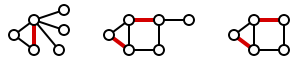
\includegraphics{Maximal-matching.png}}
    \caption{Примеры максимальных паросочетаний}
    \label{fig:Maximal-matching}
\end{figure}\\
Наибольшим паросочетанием называется наибольшее по мощности максимальное паросочетание.\\
\begin{figure}[h]
        \center{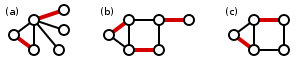
\includegraphics{Maximum-matching.png}}
    \caption{Примеры наибольших паросочетаний}
    \label{fig:Maximum-matching}
\end{figure}\\
Совершенным паросочетанием называется паросочетание, в котором каждая вершина инцидента какому-то ребру паросочетания.\\
Задача: построить наибольшее паросочетание на произвольном двудольном графе $G$.\\
$C \subseteq V(G)$ называют контролирующим множеством, если $\forall e \in E(G): C \cap e \neq \varnothing$.\\
Двойственная задача: построить минимальное контролирующее множество на произвольном двудольном графе $G$.\\
\underline{\bfЛемма}: Размер любого паросочетания не больше размера любого контролирующего множества.\\
\underline{\bfДоказательство}: Пусть $M$ - паросочетание и существует контролирующее множество $C$ такое что $|M| \textless |C| \Rightarrow \exists u \in C: \exists e_1 \neq e_2 \in M: e_1 \cap e_2 = u \Rightarrow e_1 \cap e_2 \neq \varnothing \Rightarrow$ противоречие с определением паросочетания $\Rightarrow |M| \leq |C|$.\\
\begin{figure}[h]
        \center{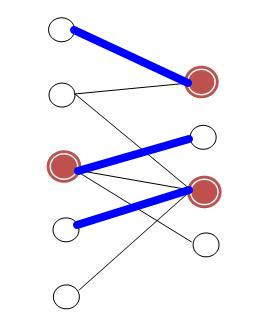
\includegraphics{Minimal-Cover.jpg}}
    \caption{Синее - максимальное паросочетание, красное - минимальное контролирующее множество}
    \label{fig:Maximal-matching and minimal-cover}
\end{figure}\\\\\\\\
\underline{\bfТеорема}: Размер наибольшего паросочетания равен размеру наименьшего контролирующего множества.\\
\underline{\bfДоказательство}: Исходя из леммы: размер наибольшего паросочетания не больше размера наименьшего контролирующего множества. Будем строить по индукции паросочетание и контролирующее его множество. $M_0 = \varnothing, C_0 = \varnothing$ - база. Пусть построено некоторое паросочетание $M_n$ на двудольном графе $G$ и множество $C_n \subseteq V(G)$ такое что $C_n$ контролирует все ребра $M_n$ и $|M_n| = |C_n|$. Если $C_n$ - контролирующее множество, то все доказано. Пусть $\exists e = uv (u \in V_1, v \in V_2)$ такое что $e \cap C_n = \varnothing$.\\
Случай 1: $\forall e' \in M: e' \cap \{u, v\} = \varnothing$. Тогда $M_{n + 1} = M_n \cup {e}, C_{n + 1} = V_1 \cap V(M_{n + 1})$.\\
Случай 2: $\exists e' \in M: e' \cap \{v\} \neq \varnothing, \forall e'' \in M: e'' \cap \{u\} = \varnothing$. Тогда определим дублера для $e': \delta(e') = e, rank(e') = rank(e) = 1$ и $M_{n + 1} = M_n, C_{n + 1} = C_n \setminus \{V_1 \cap e'\} \cup \{v\}$.\\
Случай 3: $\exists e' \in M: e' \cap \{v\} \neq \varnothing, \exists e'' \in M: e'' \cap \{u\} \neq \varnothing, rank(e'') = k$. Тогда $\delta(e') = e, rank(e') = rank(e) = k + 1$ и $M_{n + 1} = M_n, C_{n + 1} = C_n \setminus \{V_1 \cap e'\} \cup \{v\}$.\\
Случай 4: $\exists e''_k \in M: e''_k \cap \{u\} \neq \varnothing, \forall e' \in M: e' \cap \{v\} = \varnothing, rank(e''_k = k), \exists e''_{k - 1}, ..., e''_1 \in M: rank(e''_i) = i$ $ \forall i \in 1:k, \forall i \in 2:k:$ $V_1 \cap \delta(e''_i) = V_1 \cap e''_{i - 1}$. Тогда $M_{n + 1} = M_n \setminus \{e'_1, ..., e'_k\} \cup \{\delta(e'_1, ..., \delta(e'_k), e\}, C_{n + 1} = V_1 \cap V(M_{n + 1})$ и $\forall e \in E(G): rank(e) = 0, \delta(e) = \varnothing$.\\
Таким образом $|M_{n + 1}|\geq |M_n|, |C_{n + 1}| = |M_{n + 1}|$ и $C_{n + 1}$ контролирует $M_{n + 1}$.\\
В результате работы алгоритма будет построено наибольшее паросочетание $M_m$ и равное ему по размеру контролирующее множество $C_m$.\\
Примечание: не знаю насколько это неочевидно, но вот почему $C_m$ наименьшее контролирующее множество: Пусть $\exists C_{m'}: |C_{m'}| < |C_m|$ и $C_{m'}$ контролирующее множество. Тогда $|M_m| = |C_m| > |C_{m'}|$ что противоречит лемме.

\end{document}